\RequirePackage{silence} % :-\
    \WarningFilter{scrreprt}{Usage of package `titlesec'}
    %\WarningFilter{scrreprt}{Activating an ugly workaround}
    \WarningFilter{titlesec}{Non standard sectioning command detected}
\documentclass[ twoside,openright,titlepage,numbers=noenddot,%1headlines,
                headinclude,footinclude,cleardoublepage=empty,abstract=on,
                BCOR=5mm,paper=a4,fontsize=11pt
                ]{scrreprt}

%********************************************************************
% Note: Make all your adjustments in here
%*******************************************************
% ****************************************************************************************************
% classicthesis-config.tex
% formerly known as loadpackages.sty, classicthesis-ldpkg.sty, and classicthesis-preamble.sty
% Use it at the beginning of your ClassicThesis.tex, or as a LaTeX Preamble
% in your ClassicThesis.{tex,lyx} with % ****************************************************************************************************
% classicthesis-config.tex
% formerly known as loadpackages.sty, classicthesis-ldpkg.sty, and classicthesis-preamble.sty
% Use it at the beginning of your ClassicThesis.tex, or as a LaTeX Preamble
% in your ClassicThesis.{tex,lyx} with % ****************************************************************************************************
% classicthesis-config.tex
% formerly known as loadpackages.sty, classicthesis-ldpkg.sty, and classicthesis-preamble.sty
% Use it at the beginning of your ClassicThesis.tex, or as a LaTeX Preamble
% in your ClassicThesis.{tex,lyx} with \input{classicthesis-config}
% ****************************************************************************************************
% If you like the classicthesis, then I would appreciate a postcard.
% My address can be found in the file ClassicThesis.pdf. A collection
% of the postcards I received so far is available online at
% http://postcards.miede.de
% ****************************************************************************************************


% ****************************************************************************************************
% 0. Set the encoding of your files. UTF-8 is the only sensible encoding nowadays. If you can't read
% äöüßáéçèê∂åëæƒÏ€ then change the encoding setting in your editor, not the line below. If your editor
% does not support utf8 use another editor!
% ****************************************************************************************************
\PassOptionsToPackage{utf8}{inputenc}
  \usepackage{inputenc}

\PassOptionsToPackage{T1}{fontenc} % T2A for cyrillics
  \usepackage{fontenc}


% ****************************************************************************************************
% 1. Configure classicthesis for your needs here, e.g., remove "drafting" below
% in order to deactivate the time-stamp on the pages
% (see ClassicThesis.pdf for more information):
% ****************************************************************************************************
\PassOptionsToPackage{
  drafting=false,    % print version information on the bottom of the pages
  tocaligned=false, % the left column of the toc will be aligned (no indentation)
  dottedtoc=false,  % page numbers in ToC flushed right
  eulerchapternumbers=true, % use AMS Euler for chapter font (otherwise Palatino)
  linedheaders=false,       % chaper headers will have line above and beneath
  floatperchapter=true,     % numbering per chapter for all floats (i.e., Figure 1.1)
  eulermath=false,  % use awesome Euler fonts for mathematical formulae (only with pdfLaTeX)
  beramono=true,    % toggle a nice monospaced font (w/ bold)
  palatino=true,    % deactivate standard font for loading another one, see the last section at the end of this file for suggestions
  style=classicthesis % classicthesis, arsclassica
}{classicthesis}


% ****************************************************************************************************
% 2. Personal data and user ad-hoc commands (insert your own data here)
% ****************************************************************************************************
\newcommand{\myTitle}{Machine Learning in a Nutshell\xspace}
\newcommand{\mySubtitle}{An Homage to The Elements of Typographic Style\xspace}
\newcommand{\myDegree}{Doktor-Ingenieur (Dr.-Ing.)\xspace}
\newcommand{\myName}{Thimo Preis\xspace}
\newcommand{\myProf}{Put name here\xspace}
\newcommand{\myOtherProf}{Put name here\xspace}
\newcommand{\mySupervisor}{Put name here\xspace}
\newcommand{\myFaculty}{Put data here\xspace}
\newcommand{\myDepartment}{Put data here\xspace}
\newcommand{\myUni}{Put data here\xspace}
\newcommand{\myLocation}{Saarbrücken\xspace}
\newcommand{\myTime}{ \today \xspace}
\newcommand{\myVersion}{\classicthesis}
\newcommand{\myEmail}{\href{mailto:thimo.preis@posteo.de}{thimo.preis@posteo.de}}
% ********************************************************************
% Setup, finetuning, and useful commands
% ********************************************************************
\providecommand{\mLyX}{L\kern-.1667em\lower.25em\hbox{Y}\kern-.125emX\@}
\newcommand{\ie}{i.\,e.}
\newcommand{\Ie}{I.\,e.}
\newcommand{\eg}{e.\,g.}
\newcommand{\Eg}{E.\,g.}
% ****************************************************************************************************


% ****************************************************************************************************
% 3. Loading some handy packages
% ****************************************************************************************************
% ********************************************************************
% Packages with options that might require adjustments
% ********************************************************************
\PassOptionsToPackage{ngerman,american, british}{babel} % change this to your language(s), main language last
% Spanish languages need extra options in order to work with this template
%\PassOptionsToPackage{spanish,es-lcroman}{babel}
    \usepackage{babel}

\usepackage{csquotes}
\PassOptionsToPackage{%
  %backend=biber,bibencoding=utf8, %instead of bibtex
  backend=bibtex8,bibencoding=ascii,%
  language=auto,%
  style=numeric-comp,%
  %style=authoryear-comp, % Author 1999, 2010
  %bibstyle=authoryear,dashed=false, % dashed: substitute rep. author with ---
  sorting=nyt, % name, year, title
  maxbibnames=10, % default: 3, et al.
  %backref=true,%
  natbib=true % natbib compatibility mode (\citep and \citet still work)
}{biblatex}
    \usepackage{biblatex}

\PassOptionsToPackage{fleqn}{amsmath}       % math environments and more by the AMS
  \usepackage{amsmath}

% ********************************************************************
% General useful packages
% ********************************************************************
\usepackage{graphicx} %
\usepackage{scrhack} % fix warnings when using KOMA with listings package
\usepackage{xspace} % to get the spacing after macros right
\PassOptionsToPackage{printonlyused,smaller}{acronym}
  \usepackage{acronym} % nice macros for handling all acronyms in the thesis
  %\renewcommand{\bflabel}[1]{{#1}\hfill} % fix the list of acronyms --> no longer working
  %\renewcommand*{\acsfont}[1]{\textsc{#1}}
  %\renewcommand*{\aclabelfont}[1]{\acsfont{#1}}
  %\def\bflabel#1{{#1\hfill}}
  \def\bflabel#1{{\acsfont{#1}\hfill}}
  \def\aclabelfont#1{\acsfont{#1}}
% ****************************************************************************************************
%\usepackage{pgfplots} % External TikZ/PGF support (thanks to Andreas Nautsch)
%\usetikzlibrary{external}
%\tikzexternalize[mode=list and make, prefix=ext-tikz/]
% ****************************************************************************************************


% ****************************************************************************************************
% 4. Setup floats: tables, (sub)figures, and captions
% ****************************************************************************************************
\usepackage{tabularx} % better tables
  \setlength{\extrarowheight}{3pt} % increase table row height
\newcommand{\tableheadline}[1]{\multicolumn{1}{l}{\spacedlowsmallcaps{#1}}}
\newcommand{\myfloatalign}{\centering} % to be used with each float for alignment
\usepackage{subfig}
% ****************************************************************************************************


% ****************************************************************************************************
% 5. Setup code listings
% ****************************************************************************************************
\usepackage{listings}
%\lstset{emph={trueIndex,root},emphstyle=\color{BlueViolet}}%\underbar} % for special keywords
\lstset{language=[LaTeX]Tex,%C++,
  morekeywords={PassOptionsToPackage,selectlanguage},
  keywordstyle=\color{RoyalBlue},%\bfseries,
  basicstyle=\small\ttfamily,
  %identifierstyle=\color{NavyBlue},
  commentstyle=\color{Green}\ttfamily,
  stringstyle=\rmfamily,
  numbers=none,%left,%
  numberstyle=\scriptsize,%\tiny
  stepnumber=5,
  numbersep=8pt,
  showstringspaces=false,
  breaklines=true,
  %frameround=ftff,
  %frame=single,
  belowcaptionskip=.75\baselineskip
  %frame=L
}
% ****************************************************************************************************




% ****************************************************************************************************
% 6. Last calls before the bar closes
% ****************************************************************************************************
% ********************************************************************
% Her Majesty herself
% ********************************************************************
\usepackage{classicthesis}


% ********************************************************************
% Fine-tune hyperreferences (hyperref should be called last)
% ********************************************************************
\hypersetup{%
  %draft, % hyperref's draft mode, for printing see below
  colorlinks=true, linktocpage=true, pdfstartpage=3, pdfstartview=FitV,%
  % uncomment the following line if you want to have black links (e.g., for printing)
  %colorlinks=false, linktocpage=false, pdfstartpage=3, pdfstartview=FitV, pdfborder={0 0 0},%
  breaklinks=true, pageanchor=true,%
  pdfpagemode=UseNone, %
  % pdfpagemode=UseOutlines,%
  plainpages=false, bookmarksnumbered, bookmarksopen=true, bookmarksopenlevel=1,%
  hypertexnames=true, pdfhighlight=/O,%nesting=true,%frenchlinks,%
  urlcolor=CTurl, linkcolor=CTlink, citecolor=CTcitation, %pagecolor=RoyalBlue,%
  %urlcolor=Black, linkcolor=Black, citecolor=Black, %pagecolor=Black,%
  pdftitle={\myTitle},%
  pdfauthor={\textcopyright\ \myName, \myUni, \myFaculty},%
  pdfsubject={},%
  pdfkeywords={},%
  pdfcreator={pdfLaTeX},%
  pdfproducer={LaTeX with hyperref and classicthesis}%
}


% ********************************************************************
% Setup autoreferences (hyperref and babel)
% ********************************************************************
% There are some issues regarding autorefnames
% http://www.tex.ac.uk/cgi-bin/texfaq2html?label=latexwords
% you have to redefine the macros for the
% language you use, e.g., american, ngerman
% (as chosen when loading babel/AtBeginDocument)
% ********************************************************************
\makeatletter
\@ifpackageloaded{babel}%
  {%
    \addto\extrasamerican{%
      \renewcommand*{\figureautorefname}{Figure}%
      \renewcommand*{\tableautorefname}{Table}%
      \renewcommand*{\partautorefname}{Part}%
      \renewcommand*{\chapterautorefname}{Chapter}%
      \renewcommand*{\sectionautorefname}{Section}%
      \renewcommand*{\subsectionautorefname}{Section}%
      \renewcommand*{\subsubsectionautorefname}{Section}%
    }%
    \addto\extrasngerman{%
      \renewcommand*{\paragraphautorefname}{Absatz}%
      \renewcommand*{\subparagraphautorefname}{Unterabsatz}%
      \renewcommand*{\footnoteautorefname}{Fu\"snote}%
      \renewcommand*{\FancyVerbLineautorefname}{Zeile}%
      \renewcommand*{\theoremautorefname}{Theorem}%
      \renewcommand*{\appendixautorefname}{Anhang}%
      \renewcommand*{\equationautorefname}{Gleichung}%
      \renewcommand*{\itemautorefname}{Punkt}%
    }%
      % Fix to getting autorefs for subfigures right (thanks to Belinda Vogt for changing the definition)
      \providecommand{\subfigureautorefname}{\figureautorefname}%
    }{\relax}
\makeatother


% ********************************************************************
% Development Stuff
% ********************************************************************
\listfiles
%\PassOptionsToPackage{l2tabu,orthodox,abort}{nag}
%  \usepackage{nag}
%\PassOptionsToPackage{warning, all}{onlyamsmath}
%  \usepackage{onlyamsmath}


% ****************************************************************************************************
% 7. Further adjustments (experimental)
% ****************************************************************************************************
% ********************************************************************
% Changing the text area
% ********************************************************************
%\areaset[current]{312pt}{761pt} % 686 (factor 2.2) + 33 head + 42 head \the\footskip
%\setlength{\marginparwidth}{7em}%
%\setlength{\marginparsep}{2em}%

% ********************************************************************
% Using different fonts
% ********************************************************************
%\usepackage[oldstylenums]{kpfonts} % oldstyle notextcomp
% \usepackage[osf]{libertine}
%\usepackage[light,condensed,math]{iwona}
%\renewcommand{\sfdefault}{iwona}
%\usepackage{lmodern} % <-- no osf support :-(
%\usepackage{cfr-lm} %
%\usepackage[urw-garamond]{mathdesign} <-- no osf support :-(
%\usepackage[default,osfigures]{opensans} % scale=0.95
%\usepackage[sfdefault]{FiraSans}
% \usepackage[opticals,mathlf]{MinionPro} % onlytext
% ********************************************************************
%\usepackage[largesc,osf]{newpxtext}
%\linespread{1.05} % a bit more for Palatino
% Used to fix these:
% https://bitbucket.org/amiede/classicthesis/issues/139/italics-in-pallatino-capitals-chapter
% https://bitbucket.org/amiede/classicthesis/issues/45/problema-testatine-su-classicthesis-style
% ********************************************************************
% ****************************************************************************************************

% ****************************************************************************************************
% If you like the classicthesis, then I would appreciate a postcard.
% My address can be found in the file ClassicThesis.pdf. A collection
% of the postcards I received so far is available online at
% http://postcards.miede.de
% ****************************************************************************************************


% ****************************************************************************************************
% 0. Set the encoding of your files. UTF-8 is the only sensible encoding nowadays. If you can't read
% äöüßáéçèê∂åëæƒÏ€ then change the encoding setting in your editor, not the line below. If your editor
% does not support utf8 use another editor!
% ****************************************************************************************************
\PassOptionsToPackage{utf8}{inputenc}
  \usepackage{inputenc}

\PassOptionsToPackage{T1}{fontenc} % T2A for cyrillics
  \usepackage{fontenc}


% ****************************************************************************************************
% 1. Configure classicthesis for your needs here, e.g., remove "drafting" below
% in order to deactivate the time-stamp on the pages
% (see ClassicThesis.pdf for more information):
% ****************************************************************************************************
\PassOptionsToPackage{
  drafting=false,    % print version information on the bottom of the pages
  tocaligned=false, % the left column of the toc will be aligned (no indentation)
  dottedtoc=false,  % page numbers in ToC flushed right
  eulerchapternumbers=true, % use AMS Euler for chapter font (otherwise Palatino)
  linedheaders=false,       % chaper headers will have line above and beneath
  floatperchapter=true,     % numbering per chapter for all floats (i.e., Figure 1.1)
  eulermath=false,  % use awesome Euler fonts for mathematical formulae (only with pdfLaTeX)
  beramono=true,    % toggle a nice monospaced font (w/ bold)
  palatino=true,    % deactivate standard font for loading another one, see the last section at the end of this file for suggestions
  style=classicthesis % classicthesis, arsclassica
}{classicthesis}


% ****************************************************************************************************
% 2. Personal data and user ad-hoc commands (insert your own data here)
% ****************************************************************************************************
\newcommand{\myTitle}{Machine Learning in a Nutshell\xspace}
\newcommand{\mySubtitle}{An Homage to The Elements of Typographic Style\xspace}
\newcommand{\myDegree}{Doktor-Ingenieur (Dr.-Ing.)\xspace}
\newcommand{\myName}{Thimo Preis\xspace}
\newcommand{\myProf}{Put name here\xspace}
\newcommand{\myOtherProf}{Put name here\xspace}
\newcommand{\mySupervisor}{Put name here\xspace}
\newcommand{\myFaculty}{Put data here\xspace}
\newcommand{\myDepartment}{Put data here\xspace}
\newcommand{\myUni}{Put data here\xspace}
\newcommand{\myLocation}{Saarbrücken\xspace}
\newcommand{\myTime}{ \today \xspace}
\newcommand{\myVersion}{\classicthesis}
\newcommand{\myEmail}{\href{mailto:thimo.preis@posteo.de}{thimo.preis@posteo.de}}
% ********************************************************************
% Setup, finetuning, and useful commands
% ********************************************************************
\providecommand{\mLyX}{L\kern-.1667em\lower.25em\hbox{Y}\kern-.125emX\@}
\newcommand{\ie}{i.\,e.}
\newcommand{\Ie}{I.\,e.}
\newcommand{\eg}{e.\,g.}
\newcommand{\Eg}{E.\,g.}
% ****************************************************************************************************


% ****************************************************************************************************
% 3. Loading some handy packages
% ****************************************************************************************************
% ********************************************************************
% Packages with options that might require adjustments
% ********************************************************************
\PassOptionsToPackage{ngerman,american, british}{babel} % change this to your language(s), main language last
% Spanish languages need extra options in order to work with this template
%\PassOptionsToPackage{spanish,es-lcroman}{babel}
    \usepackage{babel}

\usepackage{csquotes}
\PassOptionsToPackage{%
  %backend=biber,bibencoding=utf8, %instead of bibtex
  backend=bibtex8,bibencoding=ascii,%
  language=auto,%
  style=numeric-comp,%
  %style=authoryear-comp, % Author 1999, 2010
  %bibstyle=authoryear,dashed=false, % dashed: substitute rep. author with ---
  sorting=nyt, % name, year, title
  maxbibnames=10, % default: 3, et al.
  %backref=true,%
  natbib=true % natbib compatibility mode (\citep and \citet still work)
}{biblatex}
    \usepackage{biblatex}

\PassOptionsToPackage{fleqn}{amsmath}       % math environments and more by the AMS
  \usepackage{amsmath}

% ********************************************************************
% General useful packages
% ********************************************************************
\usepackage{graphicx} %
\usepackage{scrhack} % fix warnings when using KOMA with listings package
\usepackage{xspace} % to get the spacing after macros right
\PassOptionsToPackage{printonlyused,smaller}{acronym}
  \usepackage{acronym} % nice macros for handling all acronyms in the thesis
  %\renewcommand{\bflabel}[1]{{#1}\hfill} % fix the list of acronyms --> no longer working
  %\renewcommand*{\acsfont}[1]{\textsc{#1}}
  %\renewcommand*{\aclabelfont}[1]{\acsfont{#1}}
  %\def\bflabel#1{{#1\hfill}}
  \def\bflabel#1{{\acsfont{#1}\hfill}}
  \def\aclabelfont#1{\acsfont{#1}}
% ****************************************************************************************************
%\usepackage{pgfplots} % External TikZ/PGF support (thanks to Andreas Nautsch)
%\usetikzlibrary{external}
%\tikzexternalize[mode=list and make, prefix=ext-tikz/]
% ****************************************************************************************************


% ****************************************************************************************************
% 4. Setup floats: tables, (sub)figures, and captions
% ****************************************************************************************************
\usepackage{tabularx} % better tables
  \setlength{\extrarowheight}{3pt} % increase table row height
\newcommand{\tableheadline}[1]{\multicolumn{1}{l}{\spacedlowsmallcaps{#1}}}
\newcommand{\myfloatalign}{\centering} % to be used with each float for alignment
\usepackage{subfig}
% ****************************************************************************************************


% ****************************************************************************************************
% 5. Setup code listings
% ****************************************************************************************************
\usepackage{listings}
%\lstset{emph={trueIndex,root},emphstyle=\color{BlueViolet}}%\underbar} % for special keywords
\lstset{language=[LaTeX]Tex,%C++,
  morekeywords={PassOptionsToPackage,selectlanguage},
  keywordstyle=\color{RoyalBlue},%\bfseries,
  basicstyle=\small\ttfamily,
  %identifierstyle=\color{NavyBlue},
  commentstyle=\color{Green}\ttfamily,
  stringstyle=\rmfamily,
  numbers=none,%left,%
  numberstyle=\scriptsize,%\tiny
  stepnumber=5,
  numbersep=8pt,
  showstringspaces=false,
  breaklines=true,
  %frameround=ftff,
  %frame=single,
  belowcaptionskip=.75\baselineskip
  %frame=L
}
% ****************************************************************************************************




% ****************************************************************************************************
% 6. Last calls before the bar closes
% ****************************************************************************************************
% ********************************************************************
% Her Majesty herself
% ********************************************************************
\usepackage{classicthesis}


% ********************************************************************
% Fine-tune hyperreferences (hyperref should be called last)
% ********************************************************************
\hypersetup{%
  %draft, % hyperref's draft mode, for printing see below
  colorlinks=true, linktocpage=true, pdfstartpage=3, pdfstartview=FitV,%
  % uncomment the following line if you want to have black links (e.g., for printing)
  %colorlinks=false, linktocpage=false, pdfstartpage=3, pdfstartview=FitV, pdfborder={0 0 0},%
  breaklinks=true, pageanchor=true,%
  pdfpagemode=UseNone, %
  % pdfpagemode=UseOutlines,%
  plainpages=false, bookmarksnumbered, bookmarksopen=true, bookmarksopenlevel=1,%
  hypertexnames=true, pdfhighlight=/O,%nesting=true,%frenchlinks,%
  urlcolor=CTurl, linkcolor=CTlink, citecolor=CTcitation, %pagecolor=RoyalBlue,%
  %urlcolor=Black, linkcolor=Black, citecolor=Black, %pagecolor=Black,%
  pdftitle={\myTitle},%
  pdfauthor={\textcopyright\ \myName, \myUni, \myFaculty},%
  pdfsubject={},%
  pdfkeywords={},%
  pdfcreator={pdfLaTeX},%
  pdfproducer={LaTeX with hyperref and classicthesis}%
}


% ********************************************************************
% Setup autoreferences (hyperref and babel)
% ********************************************************************
% There are some issues regarding autorefnames
% http://www.tex.ac.uk/cgi-bin/texfaq2html?label=latexwords
% you have to redefine the macros for the
% language you use, e.g., american, ngerman
% (as chosen when loading babel/AtBeginDocument)
% ********************************************************************
\makeatletter
\@ifpackageloaded{babel}%
  {%
    \addto\extrasamerican{%
      \renewcommand*{\figureautorefname}{Figure}%
      \renewcommand*{\tableautorefname}{Table}%
      \renewcommand*{\partautorefname}{Part}%
      \renewcommand*{\chapterautorefname}{Chapter}%
      \renewcommand*{\sectionautorefname}{Section}%
      \renewcommand*{\subsectionautorefname}{Section}%
      \renewcommand*{\subsubsectionautorefname}{Section}%
    }%
    \addto\extrasngerman{%
      \renewcommand*{\paragraphautorefname}{Absatz}%
      \renewcommand*{\subparagraphautorefname}{Unterabsatz}%
      \renewcommand*{\footnoteautorefname}{Fu\"snote}%
      \renewcommand*{\FancyVerbLineautorefname}{Zeile}%
      \renewcommand*{\theoremautorefname}{Theorem}%
      \renewcommand*{\appendixautorefname}{Anhang}%
      \renewcommand*{\equationautorefname}{Gleichung}%
      \renewcommand*{\itemautorefname}{Punkt}%
    }%
      % Fix to getting autorefs for subfigures right (thanks to Belinda Vogt for changing the definition)
      \providecommand{\subfigureautorefname}{\figureautorefname}%
    }{\relax}
\makeatother


% ********************************************************************
% Development Stuff
% ********************************************************************
\listfiles
%\PassOptionsToPackage{l2tabu,orthodox,abort}{nag}
%  \usepackage{nag}
%\PassOptionsToPackage{warning, all}{onlyamsmath}
%  \usepackage{onlyamsmath}


% ****************************************************************************************************
% 7. Further adjustments (experimental)
% ****************************************************************************************************
% ********************************************************************
% Changing the text area
% ********************************************************************
%\areaset[current]{312pt}{761pt} % 686 (factor 2.2) + 33 head + 42 head \the\footskip
%\setlength{\marginparwidth}{7em}%
%\setlength{\marginparsep}{2em}%

% ********************************************************************
% Using different fonts
% ********************************************************************
%\usepackage[oldstylenums]{kpfonts} % oldstyle notextcomp
% \usepackage[osf]{libertine}
%\usepackage[light,condensed,math]{iwona}
%\renewcommand{\sfdefault}{iwona}
%\usepackage{lmodern} % <-- no osf support :-(
%\usepackage{cfr-lm} %
%\usepackage[urw-garamond]{mathdesign} <-- no osf support :-(
%\usepackage[default,osfigures]{opensans} % scale=0.95
%\usepackage[sfdefault]{FiraSans}
% \usepackage[opticals,mathlf]{MinionPro} % onlytext
% ********************************************************************
%\usepackage[largesc,osf]{newpxtext}
%\linespread{1.05} % a bit more for Palatino
% Used to fix these:
% https://bitbucket.org/amiede/classicthesis/issues/139/italics-in-pallatino-capitals-chapter
% https://bitbucket.org/amiede/classicthesis/issues/45/problema-testatine-su-classicthesis-style
% ********************************************************************
% ****************************************************************************************************

% ****************************************************************************************************
% If you like the classicthesis, then I would appreciate a postcard.
% My address can be found in the file ClassicThesis.pdf. A collection
% of the postcards I received so far is available online at
% http://postcards.miede.de
% ****************************************************************************************************


% ****************************************************************************************************
% 0. Set the encoding of your files. UTF-8 is the only sensible encoding nowadays. If you can't read
% äöüßáéçèê∂åëæƒÏ€ then change the encoding setting in your editor, not the line below. If your editor
% does not support utf8 use another editor!
% ****************************************************************************************************
\PassOptionsToPackage{utf8}{inputenc}
  \usepackage{inputenc}

\PassOptionsToPackage{T1}{fontenc} % T2A for cyrillics
  \usepackage{fontenc}


% ****************************************************************************************************
% 1. Configure classicthesis for your needs here, e.g., remove "drafting" below
% in order to deactivate the time-stamp on the pages
% (see ClassicThesis.pdf for more information):
% ****************************************************************************************************
\PassOptionsToPackage{
  drafting=false,    % print version information on the bottom of the pages
  tocaligned=false, % the left column of the toc will be aligned (no indentation)
  dottedtoc=false,  % page numbers in ToC flushed right
  eulerchapternumbers=true, % use AMS Euler for chapter font (otherwise Palatino)
  linedheaders=false,       % chaper headers will have line above and beneath
  floatperchapter=true,     % numbering per chapter for all floats (i.e., Figure 1.1)
  eulermath=false,  % use awesome Euler fonts for mathematical formulae (only with pdfLaTeX)
  beramono=true,    % toggle a nice monospaced font (w/ bold)
  palatino=true,    % deactivate standard font for loading another one, see the last section at the end of this file for suggestions
  style=classicthesis % classicthesis, arsclassica
}{classicthesis}


% ****************************************************************************************************
% 2. Personal data and user ad-hoc commands (insert your own data here)
% ****************************************************************************************************
\newcommand{\myTitle}{Machine Learning in a Nutshell\xspace}
\newcommand{\mySubtitle}{An Homage to The Elements of Typographic Style\xspace}
\newcommand{\myDegree}{Doktor-Ingenieur (Dr.-Ing.)\xspace}
\newcommand{\myName}{Thimo Preis\xspace}
\newcommand{\myProf}{Put name here\xspace}
\newcommand{\myOtherProf}{Put name here\xspace}
\newcommand{\mySupervisor}{Put name here\xspace}
\newcommand{\myFaculty}{Put data here\xspace}
\newcommand{\myDepartment}{Put data here\xspace}
\newcommand{\myUni}{Put data here\xspace}
\newcommand{\myLocation}{Saarbrücken\xspace}
\newcommand{\myTime}{ \today \xspace}
\newcommand{\myVersion}{\classicthesis}
\newcommand{\myEmail}{\href{mailto:thimo.preis@posteo.de}{thimo.preis@posteo.de}}
% ********************************************************************
% Setup, finetuning, and useful commands
% ********************************************************************
\providecommand{\mLyX}{L\kern-.1667em\lower.25em\hbox{Y}\kern-.125emX\@}
\newcommand{\ie}{i.\,e.}
\newcommand{\Ie}{I.\,e.}
\newcommand{\eg}{e.\,g.}
\newcommand{\Eg}{E.\,g.}
% ****************************************************************************************************


% ****************************************************************************************************
% 3. Loading some handy packages
% ****************************************************************************************************
% ********************************************************************
% Packages with options that might require adjustments
% ********************************************************************
\PassOptionsToPackage{ngerman,american, british}{babel} % change this to your language(s), main language last
% Spanish languages need extra options in order to work with this template
%\PassOptionsToPackage{spanish,es-lcroman}{babel}
    \usepackage{babel}

\usepackage{csquotes}
\PassOptionsToPackage{%
  %backend=biber,bibencoding=utf8, %instead of bibtex
  backend=bibtex8,bibencoding=ascii,%
  language=auto,%
  style=numeric-comp,%
  %style=authoryear-comp, % Author 1999, 2010
  %bibstyle=authoryear,dashed=false, % dashed: substitute rep. author with ---
  sorting=nyt, % name, year, title
  maxbibnames=10, % default: 3, et al.
  %backref=true,%
  natbib=true % natbib compatibility mode (\citep and \citet still work)
}{biblatex}
    \usepackage{biblatex}

\PassOptionsToPackage{fleqn}{amsmath}       % math environments and more by the AMS
  \usepackage{amsmath}

% ********************************************************************
% General useful packages
% ********************************************************************
\usepackage{graphicx} %
\usepackage{scrhack} % fix warnings when using KOMA with listings package
\usepackage{xspace} % to get the spacing after macros right
\PassOptionsToPackage{printonlyused,smaller}{acronym}
  \usepackage{acronym} % nice macros for handling all acronyms in the thesis
  %\renewcommand{\bflabel}[1]{{#1}\hfill} % fix the list of acronyms --> no longer working
  %\renewcommand*{\acsfont}[1]{\textsc{#1}}
  %\renewcommand*{\aclabelfont}[1]{\acsfont{#1}}
  %\def\bflabel#1{{#1\hfill}}
  \def\bflabel#1{{\acsfont{#1}\hfill}}
  \def\aclabelfont#1{\acsfont{#1}}
% ****************************************************************************************************
%\usepackage{pgfplots} % External TikZ/PGF support (thanks to Andreas Nautsch)
%\usetikzlibrary{external}
%\tikzexternalize[mode=list and make, prefix=ext-tikz/]
% ****************************************************************************************************


% ****************************************************************************************************
% 4. Setup floats: tables, (sub)figures, and captions
% ****************************************************************************************************
\usepackage{tabularx} % better tables
  \setlength{\extrarowheight}{3pt} % increase table row height
\newcommand{\tableheadline}[1]{\multicolumn{1}{l}{\spacedlowsmallcaps{#1}}}
\newcommand{\myfloatalign}{\centering} % to be used with each float for alignment
\usepackage{subfig}
% ****************************************************************************************************


% ****************************************************************************************************
% 5. Setup code listings
% ****************************************************************************************************
\usepackage{listings}
%\lstset{emph={trueIndex,root},emphstyle=\color{BlueViolet}}%\underbar} % for special keywords
\lstset{language=[LaTeX]Tex,%C++,
  morekeywords={PassOptionsToPackage,selectlanguage},
  keywordstyle=\color{RoyalBlue},%\bfseries,
  basicstyle=\small\ttfamily,
  %identifierstyle=\color{NavyBlue},
  commentstyle=\color{Green}\ttfamily,
  stringstyle=\rmfamily,
  numbers=none,%left,%
  numberstyle=\scriptsize,%\tiny
  stepnumber=5,
  numbersep=8pt,
  showstringspaces=false,
  breaklines=true,
  %frameround=ftff,
  %frame=single,
  belowcaptionskip=.75\baselineskip
  %frame=L
}
% ****************************************************************************************************




% ****************************************************************************************************
% 6. Last calls before the bar closes
% ****************************************************************************************************
% ********************************************************************
% Her Majesty herself
% ********************************************************************
\usepackage{classicthesis}


% ********************************************************************
% Fine-tune hyperreferences (hyperref should be called last)
% ********************************************************************
\hypersetup{%
  %draft, % hyperref's draft mode, for printing see below
  colorlinks=true, linktocpage=true, pdfstartpage=3, pdfstartview=FitV,%
  % uncomment the following line if you want to have black links (e.g., for printing)
  %colorlinks=false, linktocpage=false, pdfstartpage=3, pdfstartview=FitV, pdfborder={0 0 0},%
  breaklinks=true, pageanchor=true,%
  pdfpagemode=UseNone, %
  % pdfpagemode=UseOutlines,%
  plainpages=false, bookmarksnumbered, bookmarksopen=true, bookmarksopenlevel=1,%
  hypertexnames=true, pdfhighlight=/O,%nesting=true,%frenchlinks,%
  urlcolor=CTurl, linkcolor=CTlink, citecolor=CTcitation, %pagecolor=RoyalBlue,%
  %urlcolor=Black, linkcolor=Black, citecolor=Black, %pagecolor=Black,%
  pdftitle={\myTitle},%
  pdfauthor={\textcopyright\ \myName, \myUni, \myFaculty},%
  pdfsubject={},%
  pdfkeywords={},%
  pdfcreator={pdfLaTeX},%
  pdfproducer={LaTeX with hyperref and classicthesis}%
}


% ********************************************************************
% Setup autoreferences (hyperref and babel)
% ********************************************************************
% There are some issues regarding autorefnames
% http://www.tex.ac.uk/cgi-bin/texfaq2html?label=latexwords
% you have to redefine the macros for the
% language you use, e.g., american, ngerman
% (as chosen when loading babel/AtBeginDocument)
% ********************************************************************
\makeatletter
\@ifpackageloaded{babel}%
  {%
    \addto\extrasamerican{%
      \renewcommand*{\figureautorefname}{Figure}%
      \renewcommand*{\tableautorefname}{Table}%
      \renewcommand*{\partautorefname}{Part}%
      \renewcommand*{\chapterautorefname}{Chapter}%
      \renewcommand*{\sectionautorefname}{Section}%
      \renewcommand*{\subsectionautorefname}{Section}%
      \renewcommand*{\subsubsectionautorefname}{Section}%
    }%
    \addto\extrasngerman{%
      \renewcommand*{\paragraphautorefname}{Absatz}%
      \renewcommand*{\subparagraphautorefname}{Unterabsatz}%
      \renewcommand*{\footnoteautorefname}{Fu\"snote}%
      \renewcommand*{\FancyVerbLineautorefname}{Zeile}%
      \renewcommand*{\theoremautorefname}{Theorem}%
      \renewcommand*{\appendixautorefname}{Anhang}%
      \renewcommand*{\equationautorefname}{Gleichung}%
      \renewcommand*{\itemautorefname}{Punkt}%
    }%
      % Fix to getting autorefs for subfigures right (thanks to Belinda Vogt for changing the definition)
      \providecommand{\subfigureautorefname}{\figureautorefname}%
    }{\relax}
\makeatother


% ********************************************************************
% Development Stuff
% ********************************************************************
\listfiles
%\PassOptionsToPackage{l2tabu,orthodox,abort}{nag}
%  \usepackage{nag}
%\PassOptionsToPackage{warning, all}{onlyamsmath}
%  \usepackage{onlyamsmath}


% ****************************************************************************************************
% 7. Further adjustments (experimental)
% ****************************************************************************************************
% ********************************************************************
% Changing the text area
% ********************************************************************
%\areaset[current]{312pt}{761pt} % 686 (factor 2.2) + 33 head + 42 head \the\footskip
%\setlength{\marginparwidth}{7em}%
%\setlength{\marginparsep}{2em}%

% ********************************************************************
% Using different fonts
% ********************************************************************
%\usepackage[oldstylenums]{kpfonts} % oldstyle notextcomp
% \usepackage[osf]{libertine}
%\usepackage[light,condensed,math]{iwona}
%\renewcommand{\sfdefault}{iwona}
%\usepackage{lmodern} % <-- no osf support :-(
%\usepackage{cfr-lm} %
%\usepackage[urw-garamond]{mathdesign} <-- no osf support :-(
%\usepackage[default,osfigures]{opensans} % scale=0.95
%\usepackage[sfdefault]{FiraSans}
% \usepackage[opticals,mathlf]{MinionPro} % onlytext
% ********************************************************************
%\usepackage[largesc,osf]{newpxtext}
%\linespread{1.05} % a bit more for Palatino
% Used to fix these:
% https://bitbucket.org/amiede/classicthesis/issues/139/italics-in-pallatino-capitals-chapter
% https://bitbucket.org/amiede/classicthesis/issues/45/problema-testatine-su-classicthesis-style
% ********************************************************************
% ****************************************************************************************************

\setlength{\parindent}{0pt}
\usepackage[most]{tcolorbox}
\newtcolorbox{mybox}[1]{%
	tikznode boxed title,
	enhanced,
	arc=0mm,
	interior style={white},
	attach boxed title to top center= {yshift=-\tcboxedtitleheight/2},
	fonttitle=\bfseries,
	colbacktitle=white,coltitle=black,
	boxed title style={size=normal,colframe=white,boxrule=0pt},
	title={#1}}
\newcommand{\mR}{\mathbb{R}}
\newcommand{\mJ}{\mathcal{J}}
\newcommand{\mM}{\mathcal{M}}
\newcommand{\md}{\mathrm{d}}
\newcommand{\tr}{\mathrm{Tr}}
\newcommand{\pmeasure}{\frac{\md^3 p}{(2 \pi)^3}}
 \usepackage{physics}
 \newcommand{\half}{\frac{1}{2}}
 \newcommand{\mL}{\mathcal{L}}
 \newcommand{\mV}{\mathcal{V}}
 \newcommand{\normord}[1]{\vcentcolon\mathrel{#1}\vcentcolon}
 \newcommand{\mh}{\mathsf{h}}
 \providecommand{\vcentcolon}{\mathrel{\mathop{:}}}
 \usepackage{simplewick}
 \usepackage[compat=1.1.0]{tikz-feynman}
 \newcommand{\mg}{\mathcal{g}}
 \usepackage{slashed}
 \newcommand{\munu}{_{\mu \nu}}
 \newcommand{\mG}{\mathcal{G}}
 \usepackage{savesym}
  \savesymbol{eth}
   \savesymbol{digamma}
    \savesymbol{backepsilon}
 \usepackage{amssymb}
 \newcommand{\mH}{\mathcal{H}}
 \newcommand{\mI}{\mathbb{I}}
\newcommand{\mO}{\mathcal{O}}
\newcommand{\Z}{\mathbb{Z}}
\newcommand{\bC}{\mathbb{C}}
\newcommand{\mC}{\mathcal{C}}
\usepackage{mathdots}
 \restoresymbol{ams}{eth}
  \restoresymbol{ams}{digamma}
   \restoresymbol{ams}{backepsilon}
   \newcommand{\mD}{\mathcal{D}}
\newcommand{\mA}{\mathcal{A}}
\newcommand{\mF}{\mathcal{F}}
\newcommand{\vp}{_{\vec{p}}}
\newcommand{\vz}{_{\vec{0}}}
\newcommand{\mK}{\mathcal{K}}
\newcommand{\bb}{\begin{mybox}{}} 
\newcommand{\eb}{\end{mybox}}
\newcommand{\msl}{\mathfrak{sl}}
\newcommand{\mso}{\mathfrak{so}}
\newcommand{\msu}{\mathfrak{su}}
\newcommand{\z}{\bar{z}} 
\newcommand{\h}{\bar{h}}
\newtcolorbox{example}{%
	tikznode boxed title,
	enhanced,
	arc=0mm,
	interior style={white},
	attach boxed title to top center= {yshift=-\tcboxedtitleheight/2},
	fonttitle=\bfseries,
	colbacktitle=white,coltitle=black,
	boxed title style={size=normal,colframe=white,boxrule=0pt},
	title={Example}}
\newtcolorbox{definition}{%
	tikznode boxed title,
	enhanced,
	arc=0mm,
	interior style={white},
	attach boxed title to top center= {yshift=-\tcboxedtitleheight/2},
	fonttitle=\bfseries,
	colbacktitle=white,coltitle=black,
	boxed title style={size=normal,colframe=white,boxrule=0pt},
	title={Definition}}

\newcommand{\be}{\begin{equation}}
\newcommand{\ee}{\end{equation}}
\newcommand{\bse}{\begin{equation*}}
\newcommand{\ese}{\end{equation*}}
\newcommand{\mt}{\mathbf{θ}}
\newcommand{\mX}{\mathbf{X}}
\newcommand{\mx}{\mathbf{x}}
\newcommand{\my}{\mathbf{y}}
\newcommand{\mw}{\mathbf{w}}
\newcommand{\tx}{\mathbb{x}} 
\newcommand{\tw}{\mathbb{w}}
	%********************************************************************
% Bibliographies
%*******************************************************
\addbibresource{Bibliography.bib}
\addbibresource[label=ownpubs]{AMiede_Publications.bib}
%-----------------------------------------
%My packages
%------------------------------------------
\usepackage[hyperref]{ntheorem}
\newtheorem{statements}{Statements}[chapter]
\usepackage{todonotes}
\usepackage{tikz}
\usepackage{youngtab}
\usepackage{young}
\usepackage{ytableau}
\usetikzlibrary{3d,calc,shapes.geometric}
\usepackage[makeroom]{cancel}
\usepackage{bm}



%********************************************************************
% Hyphenation
%*******************************************************
%\hyphenation{put special hyphenation here}

% ********************************************************************
% GO!GO!GO! MOVE IT!
%*******************************************************
\begin{document}
\frenchspacing
\raggedbottom
\selectlanguage{british} % american ngerman
%\renewcommand*{\bibname}{new name}
%\setbibpreamble{}
\pagenumbering{roman}
\pagestyle{plain}
%********************************************************************
% Frontmatter
%*******************************************************

%*******************************************************
% Titlepage
%*******************************************************
\begin{titlepage}
    %\pdfbookmark[1]{\myTitle}{titlepage}
    % if you want the titlepage to be centered, uncomment and fine-tune the line below (KOMA classes environment)
    \begin{addmargin}[-1cm]{-3cm}
    \begin{center}
        \large

        \hfill

        \vfill

        \begingroup
            \color{CTtitle}\spacedallcaps{\myTitle} \\ \bigskip
        \endgroup

        \spacedlowsmallcaps{\myName}\footnote{\href{mailto:thimo.preis@posteo.de}{thimo.preis@posteo.de}}
        

        \vfill

        \myTime

        \vfill

    \end{center}
  \end{addmargin}
\end{titlepage}

\cleardoublepage%*******************************************************
% Table of Contents
%*******************************************************
\pagestyle{scrheadings}
%\phantomsection
\pdfbookmark[1]{\contentsname}{tableofcontents}
\setcounter{tocdepth}{2} % <-- 2 includes up to subsections in the ToC
\setcounter{secnumdepth}{3} % <-- 3 numbers up to subsubsections
\manualmark
\markboth{\spacedlowsmallcaps{\contentsname}}{\spacedlowsmallcaps{\contentsname}}
\tableofcontents
\automark[section]{chapter}
\renewcommand{\chaptermark}[1]{\markboth{\spacedlowsmallcaps{#1}}{\spacedlowsmallcaps{#1}}}
\renewcommand{\sectionmark}[1]{\markright{\textsc{\thesection}\enspace\spacedlowsmallcaps{#1}}}
%*******************************************************
% List of Figures and of the Tables
%*******************************************************
\clearpage
% \pagestyle{empty} % Uncomment this line if your lists should not have any headlines with section name and page number
\begingroup
    \let\clearpage\relax
    \let\cleardoublepage\relax
    %*******************************************************
    % List of Figures
    %*******************************************************
    %\phantomsection
    %\addcontentsline{toc}{chapter}{\listfigurename}
    \pdfbookmark[1]{\listfigurename}{lof}
    \listoffigures

    \vspace{8ex}

    %*******************************************************
    % List of Tables
    %*******************************************************
    %\phantomsection
    %\addcontentsline{toc}{chapter}{\listtablename}
    \pdfbookmark[1]{\listtablename}{lot}
    \listoftables

    \vspace{8ex}
    % \newpage

    %*******************************************************
    % List of Listings
    %*******************************************************
    %\phantomsection
    %\addcontentsline{toc}{chapter}{\lstlistlistingname}
    \pdfbookmark[1]{\lstlistlistingname}{lol}
    \lstlistoflistings

    \vspace{8ex}

    %*******************************************************
    % Acronyms
    %*******************************************************
    %\phantomsection
    \pdfbookmark[1]{Acronyms}{acronyms}
    \markboth{\spacedlowsmallcaps{Acronyms}}{\spacedlowsmallcaps{Acronyms}}
    \chapter*{Acronyms}
    \begin{acronym}[UMLX]
        \acro{DRY}{Don't Repeat Yourself}
        \acro{API}{Application Programming Interface}
        \acro{UML}{Unified Modeling Language}
    \end{acronym}

\endgroup

%********************************************************************
% Mainmatter
%*******************************************************
\cleardoublepage
\pagestyle{scrheadings}
\pagenumbering{arabic}
\listoftodos
\chapter{Introduction}
\section{Intro to AI}
This is about considering the relationship between AI and ML.
\begin{enumerate}
	\item AI includes machine learning, but machine learning does't fully define AI. 
	\item The main point of confusion between learning and intelligence is that people assume that simply because a machine gets better at its job (\emph{learning}) it is also aware (\emph{intelligence}). Nothing supports this view of machine learning. The same phenomenon occurs when people assume that a computer is purposely causing problems for them. The computer can not assign emotions and therefore acts only upon the input provided and the instruction contained within an application to process that input. A true AI will eventually occur when computers can finally emulate the clever combination used by nature
	\begin{enumerate}
		\item \emph{Genetics}:\\
		Slow learning from one generation to the next.
		\item \emph{Teaching}:\\
		Fast learning from organized sources.
		\item \emph{Exploration}:\\
		Spontaneous learning through media and interactions with others.
	\end{enumerate}
	\item ML is only part of what a system requires to become an AI. The ML portion of the picture enables an AI to perform these tasks:
	\begin{enumerate}
		\item Adapt to new circumstances that the original developer did not envision
		\item Detect patterns in all sorts of data sources
		\item Create new behaviours based on the recognized patters
		\item Make decisions based on the success or failure of the behaviours.
	\end{enumerate}
	The use of algorithms to manipulate data is the centrepiece of ML. To prove successful, a ML sessions must use an appropriate algorithm to achieve a desired result. In addition, the data must lend itself to analysis using the desired algorithm, or it requires a careful preparation by scientists. \\
	AI encompasses many other disciplines to simulate the thought process successfully. In addition to ML, AI normally includes 
	\begin{enumerate}
		\item Natural language processing: The act of allowing language input and putting it into a form that a computer can use.
		\item Natural language understanding: The act of deciphering the language in order to act upon the meaning it provides.
		\item Knowledge representation: The ability to store information that makes fast access possible.
		\item Planning (in the form of goal seeking): The ability to use stored information to draw conclusions in near real time (almost at the moment it happens, but with a slight delay so short that only computer notices).
		\item Robotics: The ability to act upon requests from a user in some physical form
	\end{enumerate}
	
\end{enumerate}
\subsection{On governance/policy}
As scientists continue to work with a technology and turn hypotheses into theories, the technology becomes related more to engineering than science. As the rules governing a technology become clear, groups of experts work together to define these rules in written form. The result is \emph{specifications} ( a set of rules that everyone agrees upon). Eventually, implementations of the specifications become \emph{standards} that a governing body, such as the IEEE (Institute of Electrical and Electronics Engineers) or a combination of the ISO/IEC (International Organization for Standardization/international Electrotechnical Comission), manages. AI and ML have both been around long enough to create specifications, but you currently won't find any standards for either technology.

\subsection{ML}
\subsubsection{What is ML -- the schools of thought}
Statistics and ML have a lot in common and statistics represents one of the five \emph{tribes} (schools of thought) that make ML feasible. The five tribes are
\begin{enumerate}
	\item Symbolists:\\
	The origin of this tribe is in logic and philosophy. This group relies on inverse deduction to solve problems.
	\item Connectionists:\\
	The origin of this tribe is neuroscience. This group relies on backpropagation to solve problems.\\
	This tribe strives to reproduce the brain's functions using silicon instead of neurons. Essentially, each of the neurones (created as an algorithm that models the real-world counterpart) solves a small piece of the problem, and the use of many neurons in parallel solves the problem as a whole.\\
	The use of \emph{backpropagation}, or backward propagation of errors, seeks to determine the conditions under which errors are removed from networks built to resemble the human neurons by changing the \emph{weights} (how much a particular input figures into the result) and \emph{biases} (which features are selected) of the network. The goal is to continue changing the weights and biases until such time as the actual output matches the target output. At this point, the artificial neuron fires and passes its solution along to the next neuron in line. The solution created by just one neuron is only part of the whole solution. Each neuron passes information to the net neuron in line until the group of neurons creates a final output.
	\item Evolutionaries: \\
	The origin of this tribe is in evolutionary biology. This group relies on genetic programming to solve problems.\\
	The evolutionaries rely on the principles of evolution to solve problems. In other words, this strategy is based on the survival of the fittest (removing any solutions that don't match the desired output). A fitness funciton determines the viability of each function in solving a problem.\\
	Using a tree structure, the solution method looks for the best solution based on function output. The winner of each level of evolution gets to build the next-level functions. The idea is that the next level will get closer to solving the problem but may not solve it completely, which means that another level is needed. This particular tribes relies heavily on recursion and languages that strongly support recursion to solve problems. An interesting output of this strategy has been algorithms that evolve: One generation of algorithms actually builds the next generation.
	\item Bayesians:\\
	The origin of this tribe is in statistics. This group relies on probabilistic inference to solve problems.\\
	The Bayesians use various statistical methods to solve problems. Given that statistical methods can create more than one apparently correct solution, the choice of a function becomes one of determining which function has the highest probability of succeeding. For example, when using these techniques, you can accept a set of symptoms as input and decide the probability that a particular disease will result from the symptoms as output. Given that multiple diseases have the same symptoms, the probability is important because a user will see some in which a lower probability output is actually the correct output for a given circumstance.\\
	Ultimately, this tribe supports the idea of never quite trusting any hypothesis (a result that someone has given you) completely without seeing the evidence used to make it (the input the other person used to make the hypothesis). Analyzing the evidence proves or disproves the hypothesis that it supports. Consequently, it is not possible to determine which disease someone has until you test all the symptoms. One of the most recognizable outputs from this tribe is the spam filter.
	\item Analogizers:\\
	The origin of this tribe is in psychology. This group relies on kernel machines to solve problems.\\
	The analogyzers use kernel machines to recognize patterns in data. By recognizing the pattern of one set of inputs and comparing it to the pattern of a known output, you can create a problem solution. The goal is to use similarity to determine the best solution to a problem. It is the kind of reasoning that determines that using a particular solution worked in a given circumstance at some previous time; therefore, using that solution for a similar set of circumstances should also work. One of the most recognizable outputs from this tribe is recommender systems like in Amazon.
\end{enumerate}
The ultimate goal of ML is to combine the technologies and strategies embraced by the five tribes to create a single algorithm (the \emph{master algorithm}) that can learn anything.\\
ML for dummies is following Bayesian approach.
\subsubsection{What means training ?}
\begin{mybox}{}
	In machine learning you have inputs and you know the desired result. However, you do not know what function to apply to create the desired result. Training provides a learner algorithm with all sorts of examples of the desired inputs and results expected from those inputs. The learner then uses this input to create a function. In other words, training is the process whereby the learner algorithm maps a flexible function to the data. The output is typically the probability of a certain class or a numeric value.\\
	Note that we are basically talking about the function of a narrow AI, specific to one problem.
\end{mybox}
The secret to ML is generalization, the goal is to generalize the output function so that it works on data beyond the training set.\\
To create this generalized function, the learner algorithm relies on just three components:
\begin{enumerate}
	\item Representation:\\
	The learner algorithm creates a \emph{model}, which is a function that will produce a given result for specific inputs. The representation is a set of models that a learner algorithm can learn. In other words, the learner algorithm must create a model that will produce the desired results from the input data. If the learner algorithm can't perform this task, it can't learn from the data and the data is outside the hypothesis space of the learner algorithm. Part of the representation is to discover which \emph{features} (data elements within the data source) to use for the learning process.
	\item Evaluation:\\
	The learner can create more than one model. However, it does not know the difference between good and bad models. An evaluation function determines which of the models works best in creating a desired result from a set of inputs. The evaluation function scores the models because more than one model could provide the required results.
	\item Optimization:\\
	At some point, the training process produces a set of models that can generally output the right result for a given set of inputs. At this point, the training process searches through these models to determine which one works best. The best model is then output as the result of the training process.
\end{enumerate}
\subsubsection{Intriccacies with}
\begin{enumerate}
	\item Cleaning the data also lends a certain amount of artistics quality to the result. The cleaned dataset used by one scientist for ML tasks may not precisely match the cleaned datasets used by another.
	\item When working in a ML environment, you also have the problem of input data to consider. For example, the microphone found in one smartphone won't produce precisely the same input data that a microphone in another smartphone will. The characteristics of the microphones differ, yet the result of interpreting the vocal commands provided by the user must remain the same.
\end{enumerate}

\subsection{Big Data}
\section{Math basics}
\subsection{Different possible types of learning}
\subsubsection{Supervised learning}
\emph{Supervised learning} occurs when an algorithm learns from example data and associated target responses that can consist of numeric values or string labels, such as classes or tags, in order to later predict the correct response when posed with new examples. The supervised approach is indeed similar to human learning under the supervision of a teacher. The teacher provides good examples for the student to memorize, and the student then derives general rules from these specific examples.\\
You need to distinguish between regression problems, whose target is a numeric value, and classification problems, whose target is a qualitative variable, such as a class or tag. E.g. a regression task determines the average prices of houses in the Boston area, and classification tasks distinguishes between kinds of iris flowers based on their sepal and petal measures. 
\subsubsection{Unsupervised learning}
\emph{Unsupervised learning} occurs when an algorithm learns from plain examples without any associated response, leaving to the algorithm to determine the data patterns on its own. This type of algorithm tends to restructure the data into something else, such as new features that may represent a class or a new series of uncorrelated values. They are quite useful in providing humans with insights into the meaning of data and new useful inputs to supervised ML algorithms. As a kind of learning, it resembles the methods humans use to figure out that certain objects or events are from the same class, such as by observing the degree of similarity between objects. Some recommendation systems that you find on the web in the form of marketing automation are based on this type of learning. The marketing automation algorithm derives its suggestions from what you have bought in the past. The recommendations are based on an estimation of what group of customers you resemble the most and then inferring your likely preferences based on that group.

\subsubsection{Reinforcement learning}
\emph{Reinforcement learning}
occurs when you present the algorithm with examples that lack labels, as in unsupervised learning. However, you can accompany an example with positive or negative feedback according to the solution the algorithm proposes. Reinforcement learning is connected to applications for which the algorithm must make decisions (so the product is prescriptive, not just descriptive, as in unsupervised learning), and the decisions bear consequences. In the human world, it is just like learning by trial and error. Errors help you learn because they have a penalty added.\\
An interesting example occurs when computers learn to play video games by themselves. In this case, an application presents the algorithm with examples of specific situations. The application lets the algorithm know the outcome of actions it takes, and learning occurs while trying to avoid what it discovers to be dangerous and to pursue survival. The program is initially clumsy and unskilled but steadily improves with training until it becomes a champion.
\subsubsection{On the learning process}
\begin{mybox}{}
	Even though supervised learning is the most popular and frequently used, all ML algorithms respond to the same logic. The central idea is that you can represent reality using a mathematical function that the algorithm does not know in advance but can guess after having seen some data. You can express reality and all its challenging complexity in terms of unknown mathematical functions that ML algorithms find and make advantageous. This concept it the core idea for all kinds of ML algorithms.
\end{mybox}
The objective of a supervised classifier is to assign a class to an example after having examined some characteristics of the example itself. Such characteristics are called \emph{features}, and they can be both quantitative (numeric values) or qualitative (string labels). To assign classes correctly, the classifier must first examine a certain number of known examples closely (examples that already have a class assigned to them), each one accompanied by the same kinds of features as the examples that do not have classes. The training phase involves observation of many examples by the classifier that helps it learn so that it can provide an answer in terms of a class when it sees an example without a class later.
\begin{example}
	To give an idea of what happens in the training process, imagine a child learning to distinguish trees from other objects. Before the child can do so in an independent fashion, a teacher presents the child with a certain number of tree images, complete with all the facts that make a tree distinguishable from other objects of the world. Such facts could be features such as its material(wood), its parts (trunk, branches, leaves or needles, roots), and location (planted into the soil). The child produces an idea of what a tree looks like by contrasting the display of tree features with the images of other different objects, such as pieces of furniture that are made of wood but do not share other characteristics with a tree.
\end{example}
A ML classifier works the same. It builds its cognitive capabilities by creating a mathematical formulation, called a \emph{target function}, that includes all the given features ion a way that creates a function that can distinguish one class from another. Assume a target function, which can express the characteristics of a tree, to exist. In such a case, a ML classifier can look for its representation as a replica or as an approximation (a different function that works alike). Being able to express such a target function is the representation capability of the classifier.\\
The representation process takes place via \emph{mapping}, where you discover the construction of a function by observing its outputs. A successful mapping in ML is similar to a child internalizing the idea of an object. She understands the abstract rules derived from the facts of the world in an effective way so that when she sees a tree she immediately recognizes it.\\
The set of all the potential functions that the learning algorithm can figure out is called the \emph{hypothesis space}. We call the resulting classifier with all its set parameters a \emph{hypothesis}. The hypothesis space must contain all the parameter variants of all the ML algorithms that you want to try to map to an unknown function when solving a classification problem. Different algorithms can have different hypothesis spaces. What really matters is that the hypothesis space contains the target function (or its approximation, which is a different but similar function).
\begin{definition}
	In ML, someone has to provide the right learning algorithms, supply some nonlernable parameters (called \emph{hyper-parameters}), choose a set of examples to learn from, and select the features that accompany the examples. Just as a child can't always learn to distinguish between right and wrong if left alone in the world, so ML algorithms need human beings to learn successfully.
\end{definition}
Note that noise in real-world data is the norm. Many extraneous factors and errors that occur when recording data distort the values  of the features. A good ML algorithm should distinguish the signals that can map back to the target function from extraneous noise.
\subsection{Cost function}
The driving force behind optimization in ML is the response from a function internal to the algorithm, called the \emph{cost function}. You may see other terms used in some contexts, such as \emph{loss function, objective function, scoring function,} or, \emph{error function,} but the cost function is an evaluation function that measures how well the ML algorithm maps the target function that it is striving to guess. In addition, a cost function determines how well a ML algorithm performs in a supervised prediction or an unsupervised optimization problem.\\
The evaluation function works by comparing the algorithm predictions against the actual outcome recorded from the real world. Comparing a prediction against its real value using a cost function determines the algorithm's error level, keeping errors low is optimal. The cost function transmits what is actually important and meaningful for your purposes to the learning algorithm.
\begin{example}
	When the problem is to predict who will likely become ill from a certain disease, you prize algorithms that can score a high probability of singling out people who have the same characteristics and actually did become ill later. Based on the severity of the illness, you may also prefer that the algorithm wrongly chooses some people who don't get ill after all rather than miss the people who actually do get ill.
\end{example}
When an algorithm uses a cost function directly in the optimization process, the cost function is used internally. Given that algorithms are set to work with certain cost functions, the optimization objective may differ from your desired objective. In such a case, you measure the results using an external cost function that, for clarity of terminology, you call an \emph{error function} or \emph{loss function} (if it has to be minimized) or a \emph{scoring function} (if it has to be maximized).
\\
With respect to your target, a good practice is to define the cost function that works the best in solving your problem, and then to figure out which algorithms work best in optimizing it to define the hypothesis space you want to test. When you work with algorithms that don't allow the cost function you want, you can still indirectly influence their optimization process by fixing their hyper-parameters and selecting your input features with respect to your cost function. Finally, when you've gathered all the algorithm results, you evaluate them by using your chosen cost function and then decide on the final hypothesis with the best result from your chosen error function.
\begin{mybox}{}
	Deciding on the cost function is a really important and fundamental task because it determines how the algorithm behaves after learning and how it handles the problem you want to solve. Never rely on default options, but always ask yourself what you want to achieve using ML and check what cost function can best represent the achievement.
\end{mybox}
If you need to pick a cost function, ML explanations introduce a range of error functions for regression and classification, comprising root mean squared errors, log loss, accuracy, precision, recall, and area under the curve.
\subsubsection{An example: The gradient descent algorithm}
Gradient descent works out a solution by starting from a random solution when given a set of parameters (a data matrix made of features and a response). It then proceeds in various iterations using the feedback from the cost function, thus changing its parameters with values that gradually improve the initial random solution and lower the error. Even though the optimization may take a large number of iterations before reaching a good mapping, it relies on changes that improve the response cost function most (lower error) during each iteration. There can be local minima where the process may get stuck and cannot continue its descent. \\
You can visualize the optimization process as a walk in high mountains, with the parameters being the different paths to descend to the valley. A gradient descent optimization occurs at each step. At each iteration, the algorithm chooses the path that reduces error the most, regardless of the direction taken. The idea is that if steps aren't too large (causing the algorithm to jump over the target), always following the most downward direction will result in finding the lowest place. Unfortunately, this result does not always occurs because the algorithm can arrive at intermediate valleys, creating the illusion that it has reached the target. However, in most cases, gradient descent leads the ML algorithm to discover the right hypothesis for successfully mapping the problem. Given the optimization process's random initialization , running the optimization many times is good practice. This means trying different sequences of descending paths and not getting stuck in the same local minimum.\\
When working with repeated updates of its parameters base on mini-batches and single examples, the gradient descent takes the name \emph{stochastic gradient descent}.
\\
\begin{mybox}{}
	ML boils down to an optimization problem in which you look for a global minimum given a certain cost function.
\end{mybox}
\subsection{Data processing}
When operating with data within the limits of the computer's memory (RAM), you are working in \emph{core memory}. Algorithms that work with core memory are called \emph{batch algorithms}.\\
If the data set is too big to fit into the standard memory of a single computer you could the following.
\begin{enumerate} 
	\item Subsample: \\
	Data is reshaped by a selection of cases (and sometimes even features) based on statistical sampling into a more manageable, yet reduced, data matrix. Clearly, reducing the amount of data can't always provide exactly the same results as when globally analysing it. A successful subsampling must correctly use statistical sampling, by employing random or stratified sample drawings.
	\begin{definition}
		In \emph{random sampling}, you create a sample by randomly choosing the examples that appear as part of the sample. The larger the sample, the more likely he sample will resemble the original structure and variety of data, but even with few drawn examples, the results are often acceptable, both in terms of representation of the original data and for ML purposes.
	\end{definition}
	\begin{definition}
		In \emph{stratified sampling}, you control the final distribution of the target variable or of certain features in data that you deem critical for successfully replicating the characteristics of your complete data. A classic example is to draw a sample in a classroom made up of different proportions of males and females in order to guess the average height. If females are, on average, shorter than and in smaller proportion to males, you want to draw a sample that repliates the same proportion in order to obtain a reliable estimate of the average height. If you sample only males by mistake, you'll overestimate the average height. Using prior insight with sampling (such as knowing that gender can matter in height guessing) helps a lot in obtaining samples that are suitable for ML.
	\end{definition}
	After you choose a sampling strategy, you have to draw a subsample of enough examples, given your memory limitations, to represent the variety of data. Data with high dimensionality, characterized by many cases and many features, is more difficult to subsample because it needs a much larger sample, which may not even fit into your core memory.
	\item Network parallelism:\\
	Split data into multiple computers that are connected in a network. Each computer handles part of the data for optimization. You cannot split all ML algorithms into separable processes.
	\item Rely on out-of-core algorithms, which work by keeping data on the storage device and feeding it in chunks into computer memory for processing. The feeding process is called \emph{streaming}. Because the chunks are smaller than the core memory, the algorithm can handle them properly and use them for updating the ML algorithm optimization. After the update, the system discards them in favour of new chunks, which the algorithm uses for learning. This process goes on repetitively until there are no more chunks. Chunks can be small, and the process ic called \emph{mini-batching}, or they can even be constituted by just a single example, called \emph{online learning}.
\end{enumerate}
\chapter{Supervised learning}
We limit our focus to supervised and later on unsupervised learning if not specified otherwise, reinforcement learning will be treated later on.
\todo{Solve problem with bold greek letters}
\section{More formal introduction into the idea of Machine Learning}
\subsection{Problem set-up and recipe}
\label{subsec:recipeML}
Problems in ML typically involve inference about complex systems where we do not know the exact form of the mathematical model that describes the system. It is therefore not uncommon to have multiple candidate models that need to be compared.
\subsubsection{Ingredients}
Many problems in ML and data science start with the same ingredients. The first ingredient is the dataset $\mD=(\mX,\mathbf{y})$ where $\mX$ is a matrix of independent variables and $\mathbf{y}$ is a vector of dependent variables. The second is the model $f(\mx;\mt)$, which is a function $f:\mx \rightarrow y$ of the \emph{parameters} $\mt$. That is, $f$ is a function used to predict an output from a vector of input variables. 
\marginpar{Using polynomial models (i.e. polynomials of different order) in polynomial regressions, we can think of each term in the polynomial as a ’feature’ (i.e. a,b are features for $f_1(x)=a x^2+bx$) in our model, then increasing the order of the polynomial we fit increases the number of features.}
\begin{mybox}{Model class}
	To make predictions, we will consider a family of functions $f_{\alpha}(x,\mt_\alpha)$ that depend on some parameters $\mt_\alpha$. These functions represent the \emph{model class} that we are using to model the data and make predictions. Note that we choose the model class without knowing the function $f(x)$. The $f_\alpha(x;\mt_\alpha)$ encode the \emph{features} we choose to represent the data. Different models (e.g. $\alpha=1,2,3$) can contain different number of parameters, then the models have different \emph{model complexity}.
\end{mybox}
The final ingredient is the \emph{cost function} $\mC(\my,f(\mX;\mt))$ that allow us to judge how well the model performs on the observations $\my$. The model is fit by finding the value of $\mt$ that minimizes the cost function. For example, one commonly used cost function is the squared error. Minimizing the squared error cost function is known as the method of least squares, and is typically appropriate for experiments with Gaussian measurement errors.
\subsubsection{Recipe}
\begin{enumerate} 
\item The \emph{first step} in the analysis is to \emph{randomly} divide the dataset $\mD$ into two mutually exclusive groups $\mD_{train}$ and $\mD_{test}$ called the training and test sets. The fact that this must be the first step should be heavily emphasized - performing some analysis (such as using the data to select important variables) before partitioning the data is a common pitfall that can lead to incorrect conclusions. Typically, the majority of the data are partitioned into the training set (e.g. $90\%$) with the remainder going into the test set. 
\begin{mybox}{Cross evaluation}
	Therefore, to learn the parameters $\mt_\alpha$, we will train our models on a \emph{training dataset} and then test the effectiveness of the model on a \textbf{different} dataset, the \emph{test dataset}.
\end{mybox}
\item The model is fit by minimizing the cost function using only the data in the training set $\hat{\mt}= \arg \min_{θ}\{\mC(\my_{train}, f(\mX_{train};\mt) )\}$.
\item Finally, the performance of the model is evaluated by computing the cost function using the test set $\mC(\my_{test},f(\mX_{test};\hat{\mt}))$. 
\end{enumerate}
\subsection{Performance evaluation}
\label{subsec:performanceeval}
\subsubsection{Ingredients for performance evaluation}
\begin{mybox}{Measure for evaluating performance}
	The value of the cost function for the best fit model on the training set is called the \emph{in-sample error}
	\be 
	\label{eq:errorInsample}
	E_{in}=\mC(\my_{train},f(\mX_{train};\mt))
	\ee 
	and the value of the cost function on the test set is called the \emph{out-of-sample error}
	\be 
	\label{eq:errorOutsample}
	E_{out}= \mC(\my_{test},f(\mX_{test};\mt)).
	\ee 
	One of the most important observations we can make is that \textbf{the out-of-sample error is almost always greater than the in-sample error}
	\be 
	\label{eq:errorComparison}
	E_{out} \geq E_{in}.
	\ee 
	Comparison of candidate models is usually done by using $E_{out}$. The model that minimizes this out-of-sample error is chosen as the best model (i.e. model selection).
\end{mybox}
Note that once we select the best model on the basis of its performance on $E_{out}$, the real-world performance of the winning model should be expected to be slightly worse because the test data was now used in the fitting procedure.\\
Splitting the data into mutually exclusive training and test sets provides an unbiased estimate for the predictive performance of the model - this is known as \emph{cross-validation}.
\begin{mybox}{Pitfalls for performance evaluation}
	It may be at first surprising that the model that has the lowest out-of-sample error $E_{out}$ usually \emph{does not} have the lowest in-sample Error $E_{in}$. Therefore, if our goal is to obtain a model that is useful for prediction, we may not want to choose the model that provides the best explanation for the current observations. At first glance, the observation that the model providing the best explanation for the current dataset probably will not provide the best explanation for future datasets is very counter-intuitive. \\
Moreover, the discrepancy between $E_{in}$ and $E_{ou}$ becomes more and more important, as the complexity of our data, and the models we use to make predictions, grows. As the number of parameters in the model increases, we are forced to work in high-dimensional spaces. The ’curse of dimensionality’ ensures that many phenomena that are absent or rare in low-dimensional spaces become generic.
\end{mybox}
A comment on the difference between the in-and out-of-sample errors:\\
There is a fundamental difference between minimizing the in-sample error and minimizing the out-of-sample error. The underlying reason for this is that the training data may not be representative of the full data distribution. From a Bayesian point of view, as David MacKay likes to repeat: \emph{We can't make predictions without making assumptions}. Thus, it is sensible to introduce priors that reflect the fact that we are likely to be undersampled (especially in high dimensions).
\subsubsection{Another mathematical measure for performance evaluation}
\begin{mybox}{$R^2$ coefficient of determination}
	 The model performance (in-sample and out-of-sample) can be evaluated using the so-called \emph{coefficient of determination}, which is given by:
		\be
	\label{eq:errorR2}
	R^2=1-\frac{\sum_{i=1}^n \abs{y^{true}_i - y^{pred}_i}^2}{\sum_{i=1}^n \abs{y^{true}_i- \frac{1}{n} \sum_{i=1}^n y^{pred}_i}^2}.
	\ee 
Optimal performance is $R^2=1$, but it can also be negative. A constant model that always predicts the expected value of $y, ⟨y^{true}⟩,$ disregarding the input features, would get a $R^2$ score of $0$.
\end{mybox}
















\subsubsection{How to effectively do the performance evaluation}
It turns out that for complicated models studied in ML, predicting and fitting are very different things.\\
	Models that give the best fit to existing data do not necessarily make the best predictions even for simple tasks. At small sample sizes, noise can create fluctuations in the data that look like genuine patterns. Simple models (like a linear function) cannot represent complicated patterns in the data, so they are forced to ignore the fluctuations and to focus on the larger trends. 
\begin{mybox}{Overfitting}
	\label{subsubsec:overfitting}
Complex models with many parameters can capture both the global trends and noise-generated patterns at the same time. In this case, the model can be tricked into thinking that the noise encodes real information. This problem is called \emph{overfitting} and leads to a steep drop-off in predictive performance.\\
We can guard against overfitting in two ways:
\begin{enumerate}
	\item We can use less expensive models with fewer parameters, or
	\item we can collect more data so that the likelihood that the noise appears patterned decreases.
\end{enumerate}
The relative degree of overfitting: This information is contained in the difference in accuracy of our model on the training  and test datasets.
\end{mybox}
\begin{mybox}{Bias-Variance tradeoff}
	\label{subsubsec:biasvariancetradeoff}
	The \emph{bias-variance} tradeoff is used in our countermeasures against overfitting. What is it ?\\When the amount of training data is limited, one can often get better predictive power performance by using a less expressive model rather than the more complex model. The simpler model has more ’bias’ but is less dependent on the particular realization of the training dataset, i.e. less ’variance’. Therefore, even though the correct model is guaranteed to have better predictive performance for an infinite amount of training data (less bias), the training errors stemming from finite-size sampling (variance) can cause simpler models to outperform the more complex model when sampling is limited.
\end{mybox}
The bias-variance tradeoff is one of the key concepts in ML and therefore discussed quantitatively in more detail in \ref{subsubsec:biasvariancetradeoff} and qualitatively in \ref{subsubsec:biasvarianceMathematicaloneClassifier}.\\
These two concepts are now discussed in more detail, for that we introduce another quantity and then look explicitly at the components of our theory causing problems for different complexity regimes.
\begin{mybox}{Bias}
	The bias represents the best our model could do if we had an infinite amount of training data to beat down sampling noise. The bias is a property of the kind of functions, or model class, we are using to approximate $f(x)$. In general, the more complex the model class we use, the smaller the bias. However, we do not generally have an infinite amount of data. For this reason, to get best predictive power it is better to minimize the out-of-sample error, $E_{out}$, rather than the bias. 
\end{mybox}\footnote{This stems from the the law of large number. This is a theorem that describes the result of performing the same experiment a large number of times. According to the law, the average of the results obtained from a large number of trials should be close to the expected value and will tend to become closer to the expected value as more trials are performed}
How can we get a better idea of what is the true object to minimize to get bets results ? \\
The Bias-Variance tradeoff is implicitly encoded in the in-and out-of-sample errors. We will therefore draw from statistical learning theory in the following to get a better understanding of what it is we ought to be doing to achieve best practices.\\
\subsubsection{Where do the insights about how to do best practices come from ?}
The out-of-sample error will decrease with the number of data points. As the number of data points gets large, the sampling noise decreases and the training data set becomes more representative of the true distribution from which the data is drawn. For this reason, in the infinite data limit, the in-sample and out-of-sample error must approach the same value, which is called the ’bias’ of our model.

\begin{figure}[h!]
	\centering
	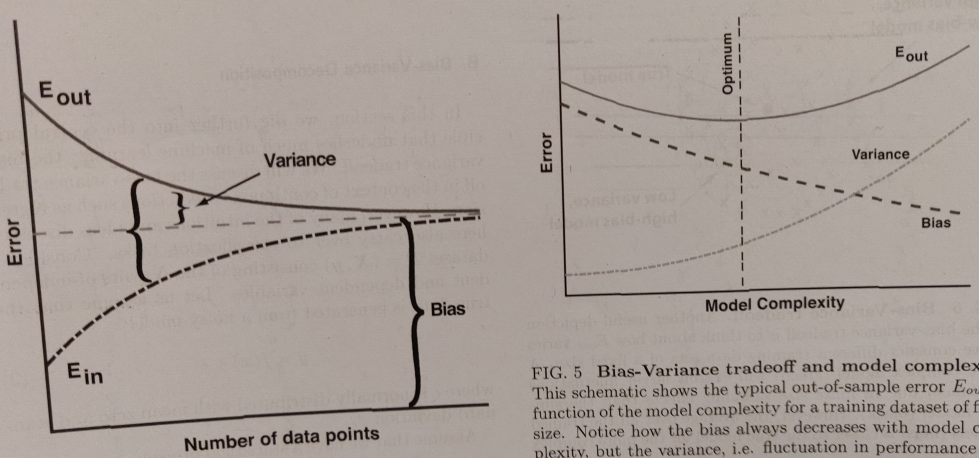
\includegraphics[width=0.7\linewidth]{gfx/InOutError.png}
	\caption{}
	\label{fig:errorbehaviour}
\end{figure}
Compare the behaviour of both errors with increasing number of data points, left graph of \ref{fig:errorbehaviour}, and the out-of-sample error with increasing model complexity, right graph of \ref{fig:errorbehaviour}. As for the left graph, we can look at the difference between the generalization ($E_{out}$) and training error ($E_{in}$), i.e. the big curly bracket representing $\abs{E_{in}-E_{out}}$. It measures how well our in-sample error reflects the out-of-sample error, and measures how much worse we would do on a new data set compared to our training data. For this reason, the difference between these errors is precisely the quantity that measures the difference between fitting and predicting. \emph{Models with a large difference between the in-sample and out-of-sample errors are said to \textbf{overfit} the data}. 
\begin{mybox}{}
	One of the lessons of statistical learning theory is that it is not enough to simply minimize the training error, because the out-of-sample error can still be large.
\end{mybox}
Considering the right graph, model  complexity is, in many cases, related to the number of parameters we are using to approximate the true function $f(x)$. If we consider a training dataset of a fixed size, $E_{out}$ will be a non-monotonic function of the model complexity, and is generally minimized for models with \emph{intermediate} complexity. The underlying reason for this is that, even though using a more complicated model always reduces the bias, at some point the model becomes too complex for the amount of training data and the generalization error becomes large due to high variance.
\begin{mybox}{}
Thus, to minimize $E_{out}$ and maximize our predictive power, it may be more suitable to use a more biased model with small variance than a less-biased model with large variance. This is is, again, the \emph{bias-variance} tradeoff we introduced above.
\end{mybox} 
Another way to understand this tradeoff is the following. Due to sampling noise from having finite size data sets, the learned models will differ for each choice of training sets. In general, more complex models need a larger amount of training data. For this reason, the fluctuations in the learned models (variance) will be much larger for the more complex model than the simpler model. However, if we consider the asymptotic performance as we increase the size of the training set (the bias), it is clear that the complex model will eventually perform better than the simpler model. Thus, depending on the amount of training data, it may \textbf{be more favourable to use a less complex, high-bias model to make predictions}.
























\section{Statistics}
Statistical modelling revolves around estimation or prediction.
\subsection{Difference between estimation and prediction}
Note first and foremost that techniques in ML tend to be more focused on prediction rather than estimation, which means that we will mostly treat prediction problems in this compendium. This is for example because an artificially intelligent agent needs to be able to recognize objects in its surroundings and predict the behaviour of its environment in order to make informed choices.\\
\subsubsection{Contrasting the two}
Estimation and prediction problems can be cast into a common conceptual framework. In both cases, we choose some observable quantity $\mx$ of the system we are studying (e.g. an interference pattern) that is related to some parameters $\mt$ (e.g. the speed of light) of a model $p(\mx|\mt)$ that describes the probability of observing $\mx$ given $\mt$.\\
Now we perform an experiment to obtain a dataset $\mX$ and use these data to fit the model. Typically,  ’fitting’ the model involves finding $\hat{\mt}$ that provides the best explanation for the data. In the case when ’fitting’ refers to the method of least squares, the estimated parameters maximize the probability of observing the data (i.e., $\hat{\mt}=\arg \max_{\mt}\{p(\mX|\mt) \}$).\\
\begin{mybox}{Estimation vs Prediction}
	\emph{Estimation problems} are concerned with the accuracy of $\hat{\mt}$, whereas \emph{prediction problems} are concerned with the ability of the model to predict new observations (i.e., the accuracy of $p(\mx|\hat{\mt})$. Although the goals of estimation and prediction are related, they often lead to different approaches.
\end{mybox}


\subsection{Mathematical motivation to presented key ideas}
We begin with an unknown function
$y = f (x)$ and fix a \emph{hypothesis set} $\mH$ consisting of all functions we are willing to consider, defined also on the domain of $f$ . This set may be uncountably infinite (e.g. if
there are real-valued parameters to fit). The choice of
which functions to include in $\mH$ usually depends on our
intuition about the problem of interest. The function
$f (x)$ produces a set of pairs $(x_i , y_i ), i = 1 . . . N$ , which
serve as the observable data. Our goal is to select a function from the hypothesis set $h \in \mH$ that approximates
$f (x)$ as best as possible, namely, we would like to find
$h \in \mH$ such that $h \approx f$ in some strict mathematical
sense which we specify below. 
\begin{mybox}{}
If this is possible, we say
that we \emph{learned} $f (x)$. 
\end{mybox}
But if the function $f (x)$ can, in
principle, take any value on \emph{unobserved inputs}, how is it
possible to learn in any meaningful sense ?\\
The answer is that learning is possible in the restricted
sense that the fitted model will probably perform approximately as well on new data as it did on the training data.
How can we evaluate the performance of our model then ?\\
As discussed in \ref{subsec:performanceeval}, once an appropriate error function $E$ is chosen for the
problem under consideration (e.g. sum of squared errors
in linear regression), we can define the in-and out-of-sample error to then minimize the out-of-sample error, with the variance-bias tradeoff in mind, to achieve robust predictions.
\subsubsection{Bias-Variance Decomposition for one Classifier}
\label{subsubsec:biasvarianceMathematicaloneClassifier}
Here we give a mathematical motivation to the bias-variance tradeoff discussed in \ref{subsubsec:biasvariancetradeoff}.\\
Consider a
dataset $\mD = (\mx, \mathbf{y})$ consisting of the $N$ pairs of independent and dependent variables. Let us assume that the
true data is generated from a noisy model
\be 
y = f (x) + \epsilon
\ee 
where $\epsilon$ is normally distributed with mean zero and standard deviation $\sigma_\epsilon$, i.e. the ’noise’.
Assume that we have a statistical procedure (e.g. least-
squares regression) for forming a predictor $f (\mx; \hat{\mathbf{θ}})$ that
gives the prediction of our model for a new data point $\mx$.
This estimator is chosen by minimizing a cost function
which we take to be the squared error
\be 
\label{eq:statCostFct}
\mC(\mathbf{y}, f(\mx; \mathbf{θ})) = \sum_i (y_i - f(x_i; \mathbf{θ}))^2.
\ee 
Therefore, the estimates for the parameters
\be 
\hat{\mathbf{θ}} =\arg \min_{θ} \mC(\mathbf{y}, f(\mx;\mathbf{θ}) )
\ee 
are a function of the dataset, $\mD$. We would obtain a
different error $\mC( \mathbf{y}_j , f (\mx_j ; \hat{\mathbf{θ}}_{\mD_j}))$ for each dataset $\mD_j =
(\mathbf{y}_j , \mx_j )$ in a universe of possible datasets obtained by
drawing $N$ samples from the true data distribution. We
denote an expectation value over all of these datasets as
$\mathbb{E}_{\mD}$.


\begin{mybox}{Errors}
	Combining these expressions,
	we see that the expected \emph{out-of-sample error}
	\be 
	 E_{out} := \mathbb{E}_{\mD,\epsilon}[\mC(\mathbf{y}, f (\mx; \hat{\mathbf{θ}}_{\mD} ))],
	\ee 
	 can be decomposed as
	 \be 
	E_{out} = \text{Bias}^2 + \text{Var} + \text{Noise},
	\ee
	with
	\begin{align*}
	\text{Noise}&=\sum_i \sigma^2_\epsilon,\; \text{Var}=\sum_i \mathbb{E}_{\mD}[(f (\mx_i ; \hat{\mathbf{θ}}_{\mD} ) − \mathbb{E}_{\mD}[f (\mx_i ; \hat{\mathbf{{θ}}}_{\mD})])^2 ],\\
	\text{Bias}^2&=\sum_i (f (\mx_i ) − \mathbb{E}_{\mD}[f ((\mx_i ;\hat{(\mathbf{θ}}_{\mD} )])^2.
	\end{align*}
	The variance measures how much our estimator fluctuates due
	to finite-sample effects and the bias measures the deviation of the expectation value of
	our estimator (i.e. the asymptotic value of our estimator
	in the infinite data limit) from the true value.
\end{mybox}
This gives us a mathematical tradeoff of the concepts discussed in \ref{subsec:performanceeval} and in particular in \ref{fig:errorbehaviour}.
\begin{mybox}{Bias-variance trade-off}
	The bias-variance tradeoff summarizes the fundamental tension in machine learning, particularly supervised
	learning, between the complexity of a model and the
	amount of training data needed to train it. Since data
	is often limited, in practice it is often useful to use a
	less-complex model with higher bias – a model whose
	asymptotic performance is worse than another model –
	because it is easier to train and less sensitive to sampling
	noise arising from having a finite-sized training dataset
	(smaller variance).
\end{mybox}
\subsubsection{Bias-Variance Decomposition for Ensembles}
\label{subsubsec:biasvarianceMathematicalEnsemble}
We will discuss the bias-variance tradeoff in the context of continuous predictions such as regression \ref{sec:linearRegression}. However, many of the intuitions and ideas discussed here also carry over to classification tasks, cf. \ref{sec:logisticRegression}. Consider a data set consisting of data $\mX_{\mL}=\{(y_j,\mx_j),j=1\dots n \}$ as above. Assume that we have a statistical procedure (e.g. OLS \ref{eq:lregOLS})) for forming a predictor $\hat{g}_{\mL}(\mx)$ that gives the prediction of our model for a new data point $\mx$ given that we trained the model using a dataset $\mL$. We will now, however, consider an ensemble of estimators $\{\hat{g}_{\mL}(\mx_i)\}$. Given a dataset $\mX_{\mL}$ and hyper-parameters $\mt$ that parametrize members of our ensemble, we will consider a procedure that deterministically generates a model $\hat{g}_{\mL}(\mx_i,\mt)$ given $\mX_{\mL}$ and $\mt$. We assume that the $\mt$ includes some random parameters that introduce stochasticity into our ensemble (e.g. an initial condition for stochastic gradient descent or a random subset of features or data points used for training.) Concretely, with a given dataset $\mL$ one has a learning algorithm $\mA$ that generates a model $\mA(\mt,\mL)$ based on a deterministic procedure which introduced stochasticity through $\mt$ in its execution on dataset $\mL$. \\
We will be concerned with the expected prediction error of the \emph{aggregate ensemble predictor}
\be 
\label{eq:biasvarianceAggregateEnsemblePredictor}
\hat{g}^A_{\mL}(\mx_i,\{\mt\} ) = \frac{1}{M} \sum_{n=1}^M \hat{g}_{\mL}(\mx_i,\mt_m).
\ee 
For future reference, let us define the mean, variance and covariance (i.e. the connected correlation function in the language of physics), and the normalized correlation coefficient of a single randomized model $\hat{g}_{\mL}(\mx,\mt_m)$ as 
\begin{align}
	\label{eq:biasvarianceDefinitionsMoments}
	\mathbb{E}_{\mL,\mt_m}[\hat{g}_{\mL}(\mx,\mt_m)] &= \mu_{\mL,\mt_m}(\mx) \nonumber \\
	\mathbb{E}_{\mL,\mt_m}[\hat{g}_{\mL}(\mx,\mt_m)^2]- \mathbb{E}_{\mL,\mt_m}[\hat{g}_{\mL}(\mx,\mt)]^2 &= \sigma^2_{\mL,\mt_m}(\mx) \nonumber \\
	\mathbb{E}_{\mL,\mt_m}[\hat{g}_{\mL}(\mx,\mt_m) \hat{g}_{\mL}(\mx,\mt_{m^\prime})] -\mathbb{E}_{\mt}[\hat{g}_{\mL}(\mx,\mt_m) ]^2 &= C_{\mL,\mt_m,\mt_{m^\prime}} (\mx) \nonumber \\
	\rho(\mx) &= \frac{C_{\mL,\mt_m,\mt_{m^\prime}}(\mx) }{\sigma^2_{\mL,\mt}}.
\end{align}
Note that the expectation $\mathbb{E}_{\mL,\mt_m}[\cdot]$ is computed over the joint distribution of $\mL$ and $\mt_m$. Also by definition, we assume $m\neq m^\prime$.\\
Now, we can, as in \ref{subsubsec:biasvarianceMathematicaloneClassifier}, define the expected generalization (out-of-sample) error for the ensemble 
\begin{align}
\label{eq:biasvarianceGeneralizationErrorEnsemble}
\mathbb{E}_{\mL,\mt_m}[C(\mX,\hat{g}^A_{\mL}(\mx))] &= \mathbb{E}_{\mL,\epsilon,\mt} \left[ \sum_i (\my_i - \hat{g}^A_{\mL} (\mx_i,\{\mt\} ))^2\right]\nonumber \\
&= Bias^2(\mx_i) + Var(\mx_i)+ \sum_i \sigma^2_{\epsilon_i},
\end{align}
where one defines the bias of an aggregate predictor 
\be 
\label{eq:biasvarianceBiasEnesemble}
Bias^2(\mx) \equiv \left(f(\mx) - \mathbb{E}_{\mL,\mt}[\hat{g}^A_{\mL} (\mx,\{\mt\}) ]\right)^2
\ee 
and the variance as
\bse 
Var(\mx) = \mathbb{E}_{\mL,\mt}\left[ (\hat{g}^A_{\mL}(\mx,\{\mt\}) - \mathbb{E}_{\mL,\mt}[\hat{g}^A_{\mL}(\mx,\{\mt\})])^2 \right]. 
\ese 
So far the calculation for ensembles is almost identical to that of a single estimator, compare \ref{subsubsec:biasvarianceMathematicaloneClassifier}.
\begin{mybox}{Crux of Bias-Variance for Ensembles}
	However, since the aggregate estimator is a sum of estimators, its variance implicitly depends on the correlations between the individual estimators in the ensemble. One finds
	\be 
	\label{eq:biasvarianceVarianceEnsembleCrux}
	Var(\mx) = \rho(\mx) \sigma^2_{\mL,\mt} + \frac{1-\rho(\mx)}{M} \sigma^2_{\mL,\mt}.
	\ee 
	This \ref{eq:biasvarianceVarianceEnsembleCrux} is the key to understanding the power of random ensembles. Notice that by using large ensembles ($M\rightarrow \infty$), we can significantly reduce the variance, and for completely random ensembles where the models are uncorrelated ($\rho(\mx)=0$), maximally suppresses the variance !\\
	Thus, reducing the aggregate predictor beats down fluctuations due to finite-sample effects. They key, as \ref{eq:biasvarianceVarianceEnsembleCrux} indicates, is to \textbf{decorrelate the models as much as possible while still using a very large ensemble.}
\end{mybox}
\begin{mybox}{What does this do to the bias ?}
One can be worried that this comes at the expense of a very large bias. This turns out not to be the case. When models in the ensemble are completely random, the bias of the aggregate predictor is just the expected bias of a single model 
\bse 
Bias^2(\mx) = (f(\mx) - \mu_{\mL,\mt})^2.
\ese 
\textbf{Thus, for a random ensemble one can always add more models without increasing the bias.}
\end{mybox}

Therefore, the correlation between models that constitute the ensemble is the key property here. It is important for two reasons. First, holding the ensemble size fixed, averaging the predictions of correlated models reduces the variance less than averaging uncorrelated models. Second, in some cases, correlations between models within an ensemble can result in an \emph{increase} in bias, offsetting any potential reduction in variance gained from ensemble averaging.\\
This will be discussed in the context of bagging  \ref{subsubsec:ensemblesBagging}.










\subsection{Mathematical set-up of every problem ever}
As described quantitatively in \ref{subsec:recipeML}, every problem in ML can be designed via a recipe which is presented now qualitatively.\\
\subsubsection{Set-up of the notation}
Suppose we are given a dataset with $n$ samples $\mD = \{(y_i,\mx^{(i)} )\}^n_{i=1}$, where $\mx^{(i)}$ is the $i$-th observation vector while $y_i$ is its corresponding (scalar) response. We assume that every sample has $p$ \emph{features}, namely,
\bse 
\mx^{(i)} \in \mR^p.
\ese  
Let $f$ be the true function/model that generated these samples via
\bse 
y_i  = f(\mx^{(i)}, \mw_{true}) + \epsilon_i,
\ese 
where $\mw_{true}\in \mR^p$ is a \emph{parameter} vector and $\epsilon_i$ is some i.i.d. white noise with zero mean and finite variance. Conventionally, we cast all samples in an $n\times p$ matrix, the \emph{design matrix}
\bse 
\mX \in \mR^{n\times p}
\ese 
with the rows 
\bse 
\mX_{i,:} = \mx^{(i)} \in \mR^p,\quad i =1,\dots,n
\ese 
being \emph{observations} and the columns
\bse 
\mX_{:,j} \in \mR^n,\quad j=1,\dots,p 
\ese 
being measured \emph{features}(i.e. feature predictors).\\
Bear in mind that this function $f$ is never known to us explicitly, though in practice we usually presume its functional form.
\begin{example}
	For example, in \emph{linear regression}, we assume
	\bse 
	y_i = f(\mx^{(i)};\mw_{true}) + \epsilon_i= \mw^T_{true} \mx^{(i)} + \epsilon_i
	\ese 
	for some unknown but fixed $\mw_{true}\in \mR^p$.
\end{example}










\subsubsection{Set-up of the problem}
We want to find a function $g$ with parameters $\mw$ fit to the data $\mD$ that can best approximate $f$. This is done when we have found a $\hat{\mw}$ such that $g(\mx;\hat{\mw})$ yields our best estimate of $f$. Now we can use this $g$ to make predictions about the response $y_0$ for a new data point $\mx_0$.\\
Therefore:\\
Fitting a given set of samples $(y_i,\mx_i)$ means relating the independent variables $\mx_i$ to their responses $y_i$. The next step is to assume some \emph{models} that might explain the measurements and measuring their performance, i.e. finding the function $g$ such that
\bse 
y_i = g(\mx_i;\mw).
\ese 
We call $g(\mx^{(i)},\mw)$ the \emph{predictor}. Recall that the optimal choice of predictor depends on, among many other things, the functions used to fit the data and the underlying noise level.
We then try to minimize the errors made in explaing the given set of measurements based on our model $g$ by tuning the parameters $\mw$. To do so, we need to first define the error function (formally called the  \emph{loss function}) that characterizes the deviation of our prediction from the actual response




\subsubsection{On statistical language}
As described above, a ML or statistics problem is defined via a optimization (minimization) problem of an error function, the solution to this is given by some estimator
\be 
\hat{\mw}_{Problem} = \arg \min_{\mw \in \mR^p} \mC(\mX, g(\mw,\my)).
\ee 
The bias (or bias function) of an estimator is the difference between this estimator's expected value and the true value of the parameter being estimated.


\subsection{Language of optimization problems}
\subsubsection{Convexity}
Recall that a set $C\subset\mR^n$ is called \emph{convex} if any  $x,y\in C$  and  $t\in [0,1]$,
\bse 
tx + (1-t) y \in C.
\ese 

In other words, every line segments joining  $x,y$  lies entirely in  $C$ .

A function $f:\mR^n \rightarrow \mR$ is called \emph{convex} if its domain $\text{dom}(f)$  is a convex set and for any  $x,y\in \text{dom}(f)$  and $ t\in[0,1]$ ,
\bse 
f(tx+(1-t)y) \leq t f(x) + (1-t) f(y).
\ese 

In other words, the function lies below the line segment joining $ f(x)$  and $ f(y)$ . This function  $f$  is called \emph{strictly convex} if this inequality holds strictly for  $x \neq y$  and  $t \in (0,1)$ .
\begin{mybox}{}
Why is convexity important? \\
\textbf{For convex functions, any local minimizer is a global minimizer}. Algorithmically, this means that in the minimization (optimization) procedure, as long as we're "going down the hill" and agree to stop when we can't go any further, then we've hit the global minimum. In addition to this, there's a menagerie of beautiful theory regarding convex duality and optimality, which gives us a way of understanding the solutions even before solving the problem itself.
\end{mybox}


\section{Overview of Bayesian Inference}
\label{sec:bayes}
Bayesian inference provides a set of principles and procedures for learning from data and for describing uncertainty.
\subsection{Language}
\begin{mybox}{Likelihood function}
	The \emph{likelihood function} 
	\be
	\label{eq:bayesLikelihoodFct}
	p(\mX|\mt)
	\ee 
	describes the probability of observing a dataset $\mX$ for a given value of the unknown parameters $\mt$. It is a function of the parameters $\mt$ with the data $\mX$ held fixed. Furthermore, it is determined by the model and the measurement noise.
\end{mybox}
\begin{mybox}{Prior distribution}
	The \emph{prior distribution} $p(\mt)$ describes any knowledge that we have about the parameters before we collect the data.
\end{mybox}
\begin{mybox}{Priors}
	\label{subsec:priors}
	There are two general classes of priors: 
	\begin{enumerate}
		\item The \emph{uninformative prior}:\\
		We choose this one if we do not have any specialized knowledge about $\mt$ before we look at the data. 
		\item The \emph{informative prior}:\\
		If we have prior knowledge, we choose an informative prior that accurately reflects the knowledge that we have about $\mt$. This one is commonly employed in ML:
	\end{enumerate}
	There is another not so important prior, the \emph{hierarchical prior}. This describes the process of choosing a hyperparameter by defining a prior distribution for it (via an uninformative prior) and then averaging the posterior distribution over all choices of the hyperparameter.
\end{mybox}
Using an informative prior tends to decrease the variance of the posterior distribution while, potentially, increasing its bias. It is beneficial if the decrease in variance is larger than the increase in bias. In high-dimensional problems, it is reasonable to assume that many of the parameters will not be strongly relevant. Therefore, many of the parameters of the model will be zero or close to zero. We can express this belief using two commonly used priors.
\begin{mybox}{Two informative priors commonly employed}
	The \emph{Gaussian prior} is used to express the assumption that many of the parameters will be small 
	\be 
	\label{eq:bayesGaussianprior}
	p(\mt|\lambda) = \prod_j \sqrt{\frac{\lambda}{2 \pi}} e^{- \lambda \theta^2_j},
	\ee
	where $\lambda$ is a \emph{hyperparameter}. The \emph{Laplace prior} is used to express the assumption that many of the parameters will be zero
	\be 
	\label{eq:bayesLaplacianprior}
	p(\mt|\lambda) = \prod_j \frac{\lambda}{2} e^{-\lambda \abs{\theta_j}}.
	\ee 
	The hyperparameter can either be chosen via a hierarchical prior employing MCMC or  by simply finding a good value of $\lambda$ using an optimization procedure (see linear regression).
\end{mybox}
Indeed, a Gaussian prior is the \emph{conjugate prior} that gives a Gaussian posterior. For a given likelihood, conjugacy guarantees the preservation of prior distribution at the posterior level.
\begin{example}
	For example, for a Gaussian (Geometric) likelihood with a Gaussian (Beta) prior, the posterior distribution is still a Gaussian (Beta) distribution.
\end{example}
\begin{mybox}{hyperparameters}
	A \emph{hyperparameter} or \emph{nuisance variable} is a parameter whose value is set before the learning process begins. By contrast, the values of other \emph{parameters} are derived via training.
\end{mybox}

\subsubsection{Connecting statistics and bayesian framework}
To connect a statistical model to the Bayesian framework, we often write the model as
\be 
\label{eq:bayesianFreqConnectionModel}
p(y|\mx,\mt) = \mathcal{N}(y|\mu(\mx),\sigma^2(\mx)).
\ee 
In other words, our model is defined by a conditional probability that depends not only on data $\mx$ but on some model parameters $\mt$.
\begin{example}
	For example, if the mean is a linear function of $\mx$ given by $\mu = \mx^T \mw$, and the variance is fixed $\sigma^2(\mx) = \sigma^2$, then $\mt=(\mw,\sigma^2)$.
\end{example}











\subsection{Calculations}
\begin{mybox}{Bayes' rule}
	The \emph{posterior distribution} $p(\mt|\mX)$ describes our knowledge about the unknown parameter $\mt$ after observing the data $\mX$. It is given via Bayes' rule
	\be 
	\label{eq:bayesrule}
	p(\mt | \mX) = \frac{p(\mX|\mt) p(\mt) }{\int \md \mt^\prime p(\mX | \mt^\prime) p(\mt^\prime)}.
	\ee
\end{mybox}
The denominator is difficult in practice such that one normally uses Markov Chain Monte Carlo (MCMC) to draw random samples from $p(\mt|\mX)$.
\subsection{Estimation}
\subsubsection{Maximum Likelihood estimation}
\label{subsubsec:bayesEstMLE}
In statistics, many problems rely on estimation of some parameters of interest.
\begin{example}
	For example, suppose we are given the height data of $20$ junior students from a regional high school, but what we are interested in is the average height of all high school juniors in the whole country. It is conceivable that the data we are given are not representative of the student population as a whole.
\end{example}
It is therefore necessary to devise a systematic way to perform reliable estimation. Here we present the \emph{maximum likelihood estimation} (MLE), and show that MLE for $\mt$ is the one that minimizes the mean squared error (MSE) used in \ref{eq:lregOLS}.
\begin{mybox}{MLE}
	Many common statistical procedures such as least-square fitting can be cast as MLE. In MLE, one chooses the parameters $\hat{\mt}$ that maximizes the likelihood (or equivalently the log-likelihood since log is a monotonic function) of the observed data $\mX$ (or equivalently $\mD$):
	\be 
	\label{eq:bayesMLE}
	\hat{\mt}= \arg \max_{\mt} \log p(\mX |\mt).
	\ee 
	In MLE we therefore choose the parameters that maximize the probability of seeing the observed data given our generative model.
\end{mybox}
Using the assumption that samples are i.i.d., we can write the \emph{log-likelihood} as 
\be 
\label{eq:bayesLogLikelihood}
l(\mt) \equiv \log p(\mD|\mt) = \sum_{i=1}^n \log p(y_i|\mx^{(i)},\mt).
\ee 
Note that the conditional dependence of the response variable $y_i$ on the independent variable $\mx^{(i)}$ in the likelihood function is made explicit since, in most applications, the observed value of data, $y_i$, is predicted based on $\mx^{(i)}$ using a model that is assumed to be a probability distribution that depends on unknown parameters $\mt$. This distribution, when endowed with $\mt$, can, as we hope, potentially explain our prediction on $y_i$. By definition, such distribution is the likelihood function \ref{eq:bayesLikelihoodFct}. We stress that this notation does \emph{not} imply $\mx^{(i)}$ is unknown, it is still part of the observed data!
\begin{mybox}{Error function}
The negative of the log-likelihood gives us the error function
\be 
\label{eq:bayesErrorFct}
E(\mt)=-l(\mt).
\ee 
\end{mybox}
\subsubsection{Maximum-a-Posteriori estimation}
\ref{eq:bayesMLE} provides the tools for computing the posterior distribution $p(\mt|\mX)$, which uses probability as a framework for expressing our knowledge about the parameters $\mt$. In most cases, however, we need to summarize our knowledge and pick a single ’best’ value for the parameters. In principle, the specific value of the parameters should be chosen to maximize a utility function. In practice, however, we usually use on of two choices:
\begin{enumerate}
	\item The posterior mean, or  \emph{Bayes estimate}
	\be 
	\label{eq:bayesBayesEstimate}
	\expval{\mt} = \int \md \mt \mt \;p(\mt |\mX),
	\ee 
	or
	\item the posterior mode, also called the \emph{maximum-a-posteriori} (MAP) estimate
	\be 
	\label{eq:bayesMAPestimate}
	\hat{\mt}_{MAP} = \arg \max_{\mt} p(\mt |\mX).
	\ee 
	This estimate gives the parameters at which the posterior probability distribution is peaked
\end{enumerate}
While the Bayes estimate minimizes the mean-squared error, MAP estimate is often used instead because it is easier to compute.
\subsubsection{Out-of-Bag estimators}
\label{subsubsec:bayesOOBestimators}
For ensemble methods, especially random forest \ref{subsec:ensemblesRandomForest}, there exists another object for estimation, the \emph{out-of-bag (OOB) estimates}.
This is discussed in more detail in \ref{subsec:ensemblesRandomForest}.
\subsection{Bayesian view on regularization}
As discussed in \ref{subsec:performanceeval}, \emph{we can't make predictions without making assumptions}. Thus, it is sensible to introduce priors that reflect the fact that we are likely to be undersampled (especially in high dimensions).\\
We can supplement an error function with a regularizer that prevents overfitting. From a Bayesian point of view, the regularization can be thought of as a prior on parameters. Minimizing the combined in-sample error $+$ regularization terms is the same as the \emph{Maximum a posteriori probability} (MAP) estimate in Bayesian regression \ref{eq:bayesMAPestimate}. Note that in a true Bayesian approach, we should not use the mode of the posterior but the average over all possible choices of parameters weighted by their posterior probability. In practice, this is often not done (for computational and practical reasons).
\subsubsection{MAP estimator in the context of regularization}
Instead of maximizing the the log-likelihood \ref{eq:bayesLogLikelihood} to obtain a good estimator \ref{eq:bayesMLE},  let us maximize the log posterior $\log p(\mt|\mD)$, which we can get via Bayes' rule \ref{eq:bayesrule}. Then, the MAP estimator becomes 
\be 
\hat{\mt}_{MAP} \equiv \arg \max_{\mt} \log p(\mD|\mt) + \log p(\mt).
\ee 
A common choice for the prior $p(\mt)$ is the Gaussian distribution. Consider the Gaussian prior \ref{eq:bayesGaussianprior} with zero mean and variance $\tau^2$, namely
\bse 
p(\mw) =\prod_j \mathcal{N}(w_j|0,\tau^2).
\ese 
Then, we can recast the MAP estimator into
\begin{align}
	\label{eq:bayesMAPestimatorGaussianPrior}
	\hat{\mt}_{MAP} &= \arg \max_{\mt} \left[ -\frac{1}{2 \sigma^2} \sum_{i=1}^n (y_i-\mw^T \mx^{(i)} )^2 - \frac{1}{2 \tau^2 } \sum_{j=1}^n w^2_j\right]\nonumber \\
	&= \arg \max_{\mt} \left[- \frac{1}{2 \sigma^2} \norm{\mX \mw -\my }^2_2 - \frac{1}{2\tau^2} \norm{\mw}^2_2\right].
\end{align}
This is used later on to cast linear regression into bayesian language, \ref{subsec:lregBayesian}.






\section{Mathematical tools}
\label{sec:math}
\subsection{Sampling methods}

\subsubsection{Empirical Bootstrapping}
\label{subsubsec:ensemblesBootstrapping}
Empirical bootstrapping is a method to enlarge a sparse dataset, we use it in bagging, cf. \ref{subsubsec:ensemblesBagging}.\\
Suppose we are given a finite set of $n$ data points $\mD=\{X_1,\dots,X_n\}$ as training samples and our job is to construct measures of confidence for our sample estimates (e.g. the confidence interval or mean-squared error of sample median estimator). To do so, one first samples $n$ points \textbf{with replacement} from $\mD$ to get a new set $\mD^{*(1)}=\{X^{*(1)}_1,\dots,X^{*(1)}_n\}$. called a \textbf{bootstrap sample}, which possibly contains repetitive elements. Then we repeat the same procedure to get in total $B$ such sets: 
\bse 
\mD^{*(1)},\dots, \mD^{*(B)}.
\ese 
The next step is to use these $B$ bootstrap sets to get the \textbf{bootstrap estimate} of the quantity of interest. For example, let $M^{*(k)}_n=$Median$(\mD^{*(k)})$ be the sample median of bootstrap data $\mD^{*(k)}$. Then we can construct the variance of the distribution of bootstrap medians as
\be 
\label{eq:ensemblesBootrapingVariance}
\hat{Var}_B(M_n)=\frac{1}{B-1} \sum_{k=1}^B \left[M^{*(k)}_n-\bar{M}^{*}_n\right]^2 = \sigma^2 \stackrel{n\rightarrow \infty}{\longrightarrow} \frac{1}{n}
\ee 
where 
\bse 
\bar{M}^{*}_n=\frac{1}{B} \sum_{k=1}^{B} M^{*(k)}_n
\ese 
is the mean of the median of all bootstrap samples.
\\
For $n\rightarrow\infty$, it was shown that the distribution of the bootstrap estimate will be a Gaussian centred around $\hat{M}_n(\mD)=$Median$(X_1,\dots,X_n)$ with standard deviation proportional to $1/\sqrt{n}$. This mean that the bootstrap distribution $\hat{M}^*_n-\hat{M}_n$ approximates fairly well the sampling distribution $\hat{M}_n-M$ from which we obtain the training data $\mD$. Note that $m$ is the median based on which the true distribution $\mD$ is generated. In other words, if we plot the histogram of $\{M^{*(k)}_n \}^B_{k=1}$, we will see that in the large $n$ limit it can be well fitted by a Gaussian which sharp peaks at $\hat{M}_n(\mD)$ and vanishing variance whose definition is given by \ref{eq:ensemblesBootrapingVariance}.

\begin{figure}[h!]
	\centering
	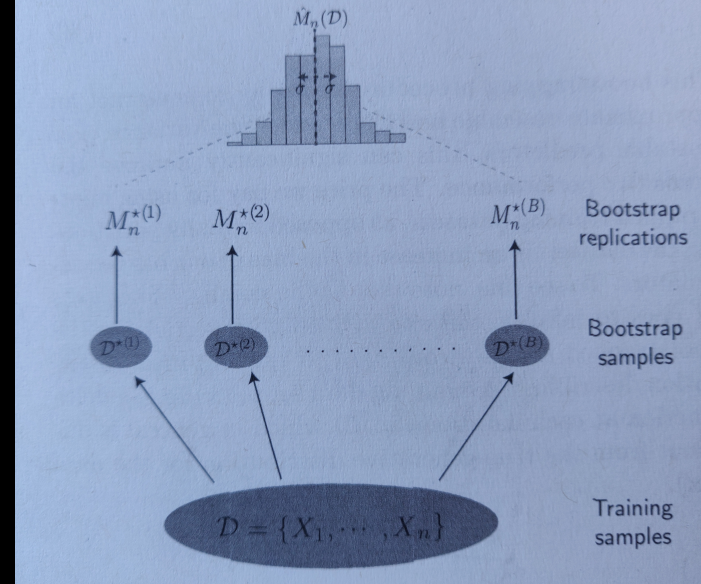
\includegraphics[width=0.7\linewidth]{gfx/Bootstrapping}
	\caption{}
	\label{fig:bootstrapping}
\end{figure}
Figure \ref{fig:bootstrapping} shows the procedure of empirical bootstrapping. 
\begin{mybox}{Bootstrapping - Summary}
	The goal is to assess the accuracy of a statistical quantity of interest, which in the main text is illustrated as the sample median $\hat{M}_m(\mD)$. We start from a given dataset $\mD$ and bootstrap $B$ size $n$ datasets $\mD^{*(1)},\dots,\mD^{*(B)}$ called the bootstrap samples. Then we compute the statistical quantity of interest on these bootstrap samples to get the median $M^{*(k)}_n$, for $k=1,\dots,B$. These are then used to evaluate the accuracy of $\hat{M}_n(\mD)$. It can be shown that in the $n\rightarrow\infty$ limit the distribution of $M^{*(k)}_n$ would be a Gaussian centred around $\hat{M}_n(\mD)$ with variance $\sigma^2$ defined by \ref{eq:ensemblesBootrapingVariance}.
\end{mybox}


\subsection{Algorithms}
\subsubsection{Decision Trees}
\label{subsubsec:ensemblesRFDecisionTree}
Decision trees are high-variance, weak classifiers that can be easily randomized, and as such, are ideally suited for ensemble-based methods.
They are employed for random forests, cf. \ref{subsec:ensemblesRandomForest}.\\
A decision tree uses a series of questions to hierarchically partition the the data. Each branch of the decision tree consists of a question that splits the data into smaller subsets with the leaves (end points) of the tree corresponding to the ultimate partitions of the data. When using decision trees for classification, the goal is to construct trees such that the partitions are informative about the class label. It is clear that more complex decision trees lead to finer partitions that give improved performance on the training set. However, this \textbf{generally leads to over-fitting}, limiting the out-of-sample performance. For this reason, in practice almost all decision trees use some form of regularization (e.g. maximum depth for the tree) to control complexity and reduce overfitting. Decision trees also have extremely high variance, and are often extremely sensitive to many details of the training data. This is not surprising since decision trees are learned by partitioning the training data. Therefore, \textbf{individual decision trees are weak classifiers.}\\
\\
However, these same properties make them ideal for incorporation in an ensemble method.\\




























\section{Gradient descent}
\label{sec:gd}
\subsection{Simple gradient descent}

As always in the context of ML, we want to minimize the cost function $E(\mathbf{θ})=\mC(\mx,g(\mathbf{θ}))$.
\begin{mybox}{Gradient descent}
The simplest gradient descent (GD) algorithm is characterized by the following \emph{update rule} for the parameters $\mathbf{θ}$. Initialize the parameters to some value $\mathbf{θ}_0$ and iteratively update the parameters according to the equation
\be
\label{eq:gdsimple}
\mathbf{v}_t = \eta_t \nabla_{θ} E(\mathbf{θ}_t),\quad \mathbf{θ}_{t+1} = \mathbf{θ}_t-\mathbf{v}_t
\ee 
where we have introduced the \emph{learning rate} $\eta_t$ (one hyperparameter of the model), that controls how big a step we should take in the direction of the gradient at time step $t$.
\end{mybox}
For sufficiently small choice of $\eta_t$, this method will converge to a \emph{local minimum} of the cost function, however this is computationally expensive. In practice, one usually specifies a ’schedule’ that decreases $\eta_t$ at long times (common schedules include power law and exponential decay in time).\footnote{Note that  Newton's method is a first-order approximation of GD method, which is not practical as it is a computationally expensive algorithm. However, Newton's method automatically adjusts the step size so that one takes larger steps in flat directions with small curvature and smaller steps in steep directions with large curavture. This gives an intuition of how to modify GD methods to get better results.}
The simple GD has the following limitations
\begin{enumerate}
\item GD finds local minima of the cost function.\\
Because in ML we are often dealing with extremely rugged landscapes with many local minima, this can lead to poor performance.
\item Gradients are computationally expensive to calculate for large datasets.
\item GD is very sensitive to choices of the learning rates.\\
Ideally, we would ’adaptively’ choose the learning rates to match the landscape.
\item GD treats all directions in parameter space uniformly.
\item GD is sensitive to initial conditions.
\item GD can take exponential time to escape saddle points, even with random initialization..
\end{enumerate}
These limitiations lead to generalized GD methods which form the backbone of much of modern DL and NN.
\subsection{Modified gradient descent}
\subsubsection{Stochastic gradient descent (SGD) with mini-batches}
\label{subsubsec:gdSGD}
\begin{mybox}{SGD}
		In SGD, we replace the actual gradient over the full data at each gradient descent step by an approximation to the gradient computed using a minibatch. This introduces stochasticity and decreases the chance that our fitting algorithm gets stuck in isolated local minima, as you cycle over all minibatches one at a time.\\
The update rule is
	\be
	\label{eq:gdstochastic}
	\mathbf{v}_t=\eta_t \nabla_{θ} E^{MB}(\mathbf{θ}),\quad \mathbf{θ}_{t+1} = \mathbf{θ}_t-\mathbf{v}_t.
	\ee 
\end{mybox}
\subsubsection{Algorithm gradient descent with momentum}
\marginpar{It has been argues that first-order methods (with appropriate initial conditions) can perform comparable to more expensive second-order methods, especially in the context of comples DL models.}
\begin{mybox}{GDM}
Introduce a ’momentum’ term into SGD which serves as a memory of the direction we are moving in parameter space. This helps the GD algorithm to gain speed in directions with persistent but small gradients even in the presence of stochasticity, while suppressing oscillations in high-curvature directions. The update rules is
\be 
\label{eq:gdmomentum}
\mathbf{v}_t = \gamma \mathbf{v}_{t-1}+\eta_t \nabla_{θ} E^{MB}(\mathbf{θ}_t), \quad \mathbf{θ}_{t+1} = \mathbf{θ}_t-\mathbf{v}_t,
\ee
where we have introduced a momentum parameter $\gamma \in [0,1]$. 
\end{mybox}
\begin{mybox}{NAG}
	A final widely used variant of gradient descent with momentum is called the Nesterov accelerated gradient (NAG). In NAG, rather than calculating the gradient at the current position, one calculates the gradient at the position momentum will carry us to at time  $t+1$ , namely, $ θ_t−γ v_{t−1}$ . Thus, the update becomes
	\be 
	\label{eq:gdNAG}
	\mathbf{v}_t = \gamma \mathbf{v}_t + \eta_t \nabla_{θ} E(\mathbf{θ}_t-\gamma \mathbf{v}_{t-1}),\quad \mathbf{θ}_{t+1} = \mt_{t}-\mathbf{v}_t.
	\ee 
\end{mybox}
\subsubsection{Methods that use the second moment of the gradient}
We would like to adaptively change the step size to match the landscape. This can be accomplished by tracking not only the gradient, but also the second moment of the gradient\footnote{Similar but avoiding the Hessian, which encodes local curvatures via second derivatives, as in Newton's method.}
\begin{mybox}{Root-mean-square propagation - RMSprop}
	In addition to keeping a running average of the first moment of the gradient, we also keep track of the second moment denoted by $\mathbf{s}_t=\mathbb{E}[\mathbf{g}^2_t]$. The update rule is 
	\be
	\label{eq:gdRMSprop}
	\mathbf{g}_t=\nabla_{θ} E(\mathbf{θ}),\; \mathbf{s}_t=\beta \mathbf{s}_{t-1} + (1-\beta) \mathbf{g}^2_t,\; \mathbf{θ}_{t+1}=\mathbf{θ}_t - \eta_t \frac{\mathbf{g}_t}{\sqrt{\mathbf{s}_t+\epsilon}},
		\ee 
		where $\beta$ controls the averaging time of the second moment and is typically taken to be about $\beta=0.9$, $\eta_t$ is typically chosen to be $10^{-3}$, and $\epsilon\propto 10^{-8}$ is a small regularization constant to prevent divergencies. It is clear from this formula that the learning rate is reduced in directions where the gradient is consistently large.
\end{mybox}
\begin{mybox}{ADAM}
	In ADAM, we keep a running average of both the first and second moment of the gradient and use this information to adaptively change the learning rate for different parameters. In addition to keeping a running average of the second moments of the gradient (i.e $\mathbf{m}_t= \mathbb{E}[\mathbf{g}_t], \mathbf{s}_t=\mathbb{E}[\mathbf{g}^2_t]$), ADAM performs an additional bias correction to account for the fact that we are estimating the first two moments of the gradient using a running average (denoted by the hat in the update rule). The update rule is given by (where multiplication and division are once again understood to be element-wise operations)
	\begin{align}
		\label{eq:gdADAM}
		\mathbf{g}_t &= \nabla_{θ} E(\mathbf{θ}), \quad \mathbf{m}_t =\beta_1 \mathbf{m}_{t-1} + (1-\beta_1) \mathbf{g}_t, \\
		\mathbf{s}_t &=\beta_2 \mathbf{s}_{t-1} + (1-\beta_2) \mathbf{g}^2_t,\quad \hat{\mathbf{m}}_t = \frac{\mathbf{m}}{1-(\beta_1)^t},\nonumber \\
		\hat{\mathbf{s}}_t &= \frac{\mathbf{s}_t}{1-(\beta_2)^t},\quad \mathbf{θ_{t+1}} = \mathbf{θ}_t - \eta_t \frac{\hat{\mathbf{m}}}{\sqrt{\hat{\mathbf{s}}_t} +\epsilon}\nonumber,
	\end{align}
where $\beta_1$ and $\beta_2$ set the memory lifetimes of the first and second moment (typically $\beta_{1,2} =\{0.9,0.99\}$ respectively, $\epsilon,\eta_t$ are same as in RMSprop).
\end{mybox}
The learning rates for RMSprop and ADAM can be set significantly higher than other methods due to their adaptive step sizes. For this reason, ADAM and RMSprop tend to be much quicker at navigating the landscape than simple momentum based methods.\footnote{Note that in some cases trajectories might not end up at the global minimum. This kind of landscape structure is generic in high-dimensional spaces where saddle points proliferate.}
\subsection{Practical tips for using GD}
Employ these tips for getting the best performance from GD based algorithms, especially in the context of deep neural networks (DNN)
\begin{enumerate}
	\item Randomize the data when making mini-batches.\\
	Otherwise, the GD method can fit spurious correlations resulting from the order in which data is presented.
	\item Transform your inputs.\\
	One simple trick for minimizing problems in difficult landscapes is to standardize the data by subtracting the mean and normalizing the variance of input variables. Whenever possible, also decorrelate the inputs. 
	\item Monitor the out-of-sample performance.\\
	Always monitor the performance of your model on a validation set (a small portion of the training data that is held out of the training process to serve as a proxy for the test set). If the validation error starts increasing then the model is beginning to overfit. Terminate the learning process. This \emph{early stopping} significantly improves performance in many settings.
	\item Adaptive optimization methods do not always have good generalization.\\
	Recent studies have shown that adaptive methods such as ADAM, RMSprop , and AdaGrad tend to have poor generalization to SGD or SGD with momentum, particularly in the high-dimensional limit (i.e. the number of parameters exceeds the number of data points). Although it is not clear at this state why sophisticated methods (e.g. ADAM, RMSprop, AdaGrad)  perform so well in training DNN such as generative adversarial networks (GANs), simpler procedures like properly-tuned plain SGD may work equally well or better in some applications.
\end{enumerate}







\section{Linear regression}
\label{sec:linearRegression}

\subsection{Least-square regressions -frequentist}
We'll consider ordinary least squares regression problem in which the "error function" is defined as the square from the deviation of our linear predictor to the true response. 
\begin{mybox}{OLS}
\emph{Ordinary least squares linear regression} (OLS) is defined as the minimization of the $L_2$ norm of the difference between the response $y_i$ and the predictor $g(\mx^{(i)};\textbf{w})=\textbf{w}^T \mx^{(i)}$:
\be 
\label{eq:lregOLS}
\min_{\textbf{w} \in \mR^p} \norm{\mX \textbf{w} -\my}^2_2 = \min_{\textbf{w} \in \mR^p}\sum_{i=1}^n (\mw^T \mx^{(i)} - y_i)^2.
\ee
Where \ref{eq:lregOLS} is the minimization of the loss function of OLS.\\
We are looking to find the parameters $\mw$ which minimize the $_2$ error. Geometrically speaking, the predictor function $g$ defines a hyperplane in $\mR^p$. Minimizing the least squares error is therefore equivalent to minimizing the sum of all projections (i.e. residuals) for all points$\mx^{(i)}$ to this hyperplane. If $\rank (\mX)=p$ , namely, the feature predictors  $\mX_{:,1},\dots,\mX_{:,p}$  are linearly independent, then there exists unique solution to this problem, which we denote as $\hat{\mw}_{LS}$:
\be 
\label{eq:lregOLSsolution}
\hat{\mw}_{LS} = \arg \min_{\mw \in \mR^p} \norm{\mX \mw - \my}^2_2 = (\mX^T \mX )^{-1} \mX^T \my,
\ee 
where we have assumed that $\mX^T\mX$ is inertible, which is often the case when $n\gg p$ (i.e. method works if number of data points exceeds number of features). The best fit of our data $\mX$ is
\be 
\label{eq:lregOLbestfit}
\hat{\my} = \mX \hat{\mw}_{LS} = \underbrace{\mX (\mX^T \mX)^{-1} \mX^T}_{\equiv P_{\mX}},
\ee 
where $P_{\mX}$ is the projection matrix which acts on $\my$ and projects it onto the column space of $\mX$, which is spanned by the predictors $\mX_{:,1},\dots,\mX_{:,p}$.
\end{mybox}
Note how we found the optimal solution $\hat{\mw}_{LS}$ in one shot, without doing any sort of iterative optimization.\\
What are the errors of OLS such that we can evaluate its performance according to \ref{subsec:performanceeval} ?\footnote{As we have seen, the difference between learning and fitting lies in the prediction on ’unseen’ data.}\\
We find that the average \emph{generalization error} for this method to be
\be 
\abs{\bar{E}_{in}-\bar{E}_{out}} = \sigma^2 \abs{(1-\frac{p}{n}) -(1+\frac{p}{n})}= 2 \sigma^2 \frac{p}{n}.
\ee 
\begin{mybox}{}
	This implies: If we have $p\gg n$ (i.e. high-dimensional data), the generalization error is extremely large, meaning the model is not learning. Even when we have $p\approx n$, we might still not learn well due to the intrinsic noise $\sigma^2$.
\end{mybox}
One way to ameliorate this is to use regularization. We will mainly focus on two forms of regularization which are introduced in the following:\\
the first one employs an $L_2$ penalty and is called \emph{Ridge regression}, while the second uses an $L_1$ penalty and is called $LASSO$.
\subsection{Regularized Least-square regressions-frequentist}
Due to poor generalization, regularization is necessary, in particular  in the \emph{high-dimensional limit} ($p\gg n$). Regularization typically leads to better generalization. 
\begin{mybox}{Idea behind regularization}
	Due to the equivalence between the constrained and penalized form of regularized regression, we can regard the regularized regression problem as an un-regularized problem but on a \emph{constrained set of parameters}. Since the size of the allowed parameter space (e.g. $\mw \in \mR^p$ when un-regularized vs. $\mw \in C \subset \mR^p$ when regularized) is roughly a proxy for model complexity, solving the regularized problem is in effect \textbf{solving the un-regularized problem with a smaller model complexity class}. This implies that we are \textbf{less likely to overfit}.
\end{mybox}
Why is that so ?\\
Let's say you are a young Physics student taking a laboratory class where the goal of the experiment is to measure the behaviour of several different pendula and use that to predict the formula (i.e. model) that determines the period of oscillation. In you investigation you would probably recod many things in an effort to give yourself the best possible chance of determining the unknown relationship, perhaps writing down the temperature of the room, any air currents, if the table were vibrating, etc. What you have done is create a high-dimensional dataset for yourself. However you actually possess an even higher-dimensional dataset than you probably would admit to yourself, e.g. whether it is Alice's birthday or whether you found a penny this morning, but you almost assuredly haven't written these down in your notebook. Why not ? The reason is because \emph{you entered the classroom with strongly held \textbf{prior beliefs} that none of those things affect the physics which takes place in that room}. What is serving you here is the \emph{intuition} that probably only a few things matter in the physics of pendula. Hence again you are approaching the experiment with prior beliefs about how many features you will need to pay attention to in order to predict what will happen when you swing an unknown pendulum.\\
The point is that we live in a high-dimensional world of information and while we have good intuition about what to write down in our notebook for well-known problems, often in the field of ML we cannot say with any confidence a priori \emph{what} the small list of things to write down will be, but we can at least \textbf{use regularization to help us enforce that the list not be too long} so that we don't end up predicting that the period of a pendulum depends on Bob having a cold on Wednesdays.
\subsubsection{Ridge-Regression}
\begin{mybox}{Ridge-Regression}
	We now add to the least squares loss function a \emph{regularizer} defined as as the $L_2$ norm of the parameter vector we wish to optimize over. In Ridge-Regression, the regularization penalty is taken to be the $L_2$-norm of the parameters 
	\be 
	E_{Ridge} = \lambda \norm{\mw}^2_2 = \lambda \mw^T\mw = \lambda \sum_{\gamma=1}^p w_\gamma w_\gamma.
	\ee 
	Thus, the model is fit by minimizing the sum of the in-sample error and the regularization term
	\be 
	\label{eq:lregRidge}
	\hat{\mw}_{Ridge} (\lambda) = \arg \min_{\mw \in \mR^p}\left(\norm{\mX \mw - \my}^2_2 + \lambda \norm{\mw}^2_2\right)
	\ee 
	Notice that the parameter $\lambda$ controls how much we weigh the fit and regularization term.
	The solution/estimate is found by differentiating w.r.t $\mw$
	\be 
	\label{eq:lregRidgeSol}
	\hat{\mw}_{Ridge}(\lambda)=\frac{\hat{\mw}_{LS}}{1+\lambda} 
	\ee 
	where the  equality via \ref{eq:lregOLSsolution} holds for orthogonal $\mX$. This implies that the ridge estimate is merely the least squares estimate scaled by a factor $(1+\lambda)^{-1}$.
	This problem is equivalent to the following \emph{constrained} optimization problem
	\be 
	\hat{\mw}_{Ridge}(t) ) \arg \min_{\mw \in \mR^p: \norm{\mw}^2_2 \leq t} \norm{\mX \mw -\my}^2_.2.
	\ee 
	Thus, by adding a regularization term, $\lambda \norm{\mw}^2_2$, to our least squares loss function, we are effectively constraining the magnitude of the parameter vector learned from the data. The solution
\end{mybox}
One can furthermore derive a relation (via singular value decomposition (SVD) on X) between the fitted vector $\hat{\my}=\mX\hat{\mw}_{Ridge}$ and the prediction made by least squares linear regression
\be 
\hat{y}_{Ridge} =\mX \hat{\mw}_{Ridge} \leq \mX \hat{\my} \equiv \hat{\my}_{LS}.
\ee 
It is clear that in order to compute the fitted vector $\hat{\my}$, both Ridge and least squares linear regression have to project $\my$ to the column space of $\mX$. The only difference is that Ridge regression further shrinks each basis component $j$ by a factor $d^2_j/(d^2_j+\lambda)$, where $d_1\geq d_2\geq \dots d_p \geq 0$ are the singular values of $\mX$.
\begin{mybox}{}
	It is considered good practice to always check the performance for the given model and data as a function of $\lambda$.
\end{mybox}
If increasing $\lambda$  simply degrades performance, we are most likely not undersampled.
\subsubsection{LASSO and Sparse Regression}
\begin{mybox}{LASSO}
	Now we add an $L_1$ regularization penalty, conventionally called ’least absolute shrinkage and selection operator’ (LASSO). The penalty is the $L_1$-norm of the parameters (sum of absolute values of parameters)
	\be 
	E_{LASSO}= \lambda \norm{\mw}_1 = \lambda \sum_{\gamma=1}^p \abs{\mw_\gamma}
	\ee 
	LASSO in the penalized form is defined by the following regularized regression problem
	\be 
	\label{eq:lregLASSO}
	\hat{\mw}_{LASSO}(\lambda) = \arg \min_{\mw \in \mR^p} \norm{\mX \mw - \my }^2_2 + \lambda \norm{\mw}_1.
	\ee 
	Obtaining a solution is not that easy, assuming $\mX$ to be orthogonal one finds a so-called threshold function (compare \ref{fig:lassovsridge})
	\be 
	\label{eq:lregLASSOSol}
	\hat{w}^{LASSO}_j(\lambda)= \text{sign}(\hat{w}^{LS}_j)\left[\abs{\hat{w}^{LS}_j}-\lambda\right]_+
	\ee 
	where $(x)_+$ denotes the positive part of $x$ and $\hat{w}^{LS}_j$ is the $j$th component of \ref{eq:lregOLSsolution}.\\
	In general, LASSO tends, in contrast to Ridge, to given sparse solutions, meaning many components of $\hat{\mw}_{LASSO}$ are zero. Looking at the behaviour of weights of LASSO and Ridge depending on the regularization parameter, one observes that LASSO, unlike Ridge, sets feature weights to zero leading to sparsity.
\end{mybox}
\begin{figure}[h!]
	\centering
	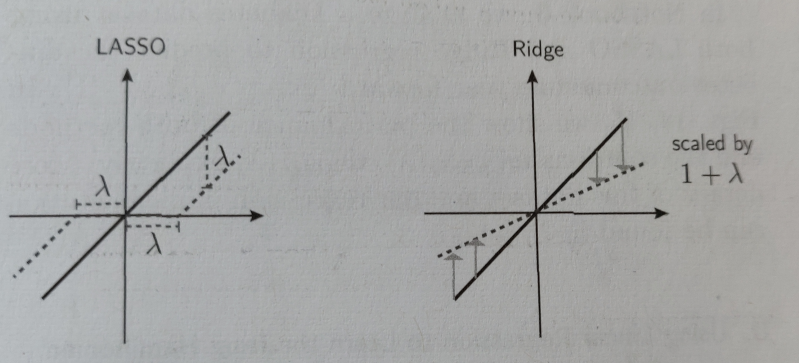
\includegraphics[width=0.7\linewidth]{gfx/LassoVsRidge}
	\caption{}
	\label{fig:lassovsridge}
\end{figure}
\begin{mybox}{On the hyperparameter}
	The regularization parameter $\lambda$ affects the weights (features) the model (LASSO, Ridge) learns on a data set.
\end{mybox}

\subsubsection{A note on LASSO and Ridge}
Note that both LASSO and Ridge regression are convex in  $\mw$ . What's more, Ridge is actually a strictly convex problem (assuming  $\lambda >0$ ) due to presence of $L_2$ penality. In fact, this is always true regardless of  $\mX$  and so the ridge regression solution is always well-defined.

In contrast, LASSO is not always strictly convex and hence by convexity theory, it need not have a unique solution. The LASSO solution is unique under general conditions, for example, when  $\mX$  has columns in general position. To mitigate this, one can define a modified problem called the elastic net such that the function we want to minimize is always strictly convex:
\bse 
\min_{\mw \in \mR^p}\norm{\mX \mw -\my}^2_2 + \lambda \norm{\mw}_1+\delta \norm{\mw}^2_2
\ese 
where  $λ,δ\geq 0$  are regularization parameters. Now aside from uniqueness of the solution, the elastic net combines some of the desirable properties (e.g. prediction) of ridge regression with the sparsity properties of the LASSO.
\subsubsection{Another note being a general comment on regularization}
Comparing the performance of OLS, LASSO and Ridge for the $1D$ Ising model via the coefficient of determination \ref{eq:errorR2} by looking at the parameter space of the hyperparameter $\lambda$, one can draw the following conclusions.\\
Choosing whether to use Ridge or LASSO regression turns out to be similar to fixing gauge degrees of freedom.
\begin{mybox}{Picking a regularization scheme}
	Different regularization schemes can lead to learning equivalent models but in different ’gauges’. Any information we have about the symmetry of the unknown model that generated the data should be reflected in the definition of the model and the choice of regularization.
\end{mybox}

\subsubsection{A general perspective on regularizers}
\begin{mybox}{On the hyperparameter}
	The \textbf{hyperparameter} $\lambda$ involved in e.g. LASSO and Ridge is usually predetermined, which means that it is not part of the regression process. Our learning performance and solution depends strongly on $\lambda$, thus it is vital to choose it properly. As discussed in \ref{subsec:priors}, one approach is to assume an \emph{uninformative prior} on the hyper-parameters, $p(\lambda)$, and average the posterior over all choices of $\lambda$ following this distribution. However, this comes with a large computational cost. Therefore, is is simpler to choose the regularization parameter through some optimization procedure.
\end{mybox}






\subsection{Bayesian formulation of linear regression}
\label{subsec:lregBayesian}
In the formal statistical treatment of regression, the goal is to estimate the \emph{conditional expectation} of the depndent variable given the value of the independent variable (sometimes called the covariate). To connect linear regression to the Bayesian framework, we use \ref{eq:bayesianFreqConnectionModel}. In combination with \ref{eq:bayesLogLikelihood}, we get
\bse 
l(\mt)=-\frac{1}{2\sigma^2} \sum_{i=1}^n(y_i-\mw^T \mx^{(i)})^2-\frac{n}{2} \log(2 \pi  \sigma^2) = -\frac{1}{2\sigma^2} \norm{\mX \mw -\my}^2_2 + const.
\ese
\begin{mybox}{} 
By comparing this with \ref{eq:lregOLSsolution}, it is clear that 
 performing least squares is the same as maximizing the log-likelihood of this model.
\end{mybox}

 \subsubsection{Regularization }
 What about adding regularization?
 \begin{mybox}{}
 The MAP estimate  \ref{eq:bayesMAPestimate} corresponds to regularized linear regression, where the choice of prior determines the type of regularization.
 \end{mybox}
The equivalence between MAP estimation with a Gaussian prior and Ridge regression is established by comparing \ref{eq:bayesMAPestimatorGaussianPrior} and Ridge regression \ref{eq:lregRidgeSol} with $\lambda \equiv \sigma^2/\tau^2$. An analogous derivation holds for LASSO \todo{todo ?}.

\subsection{Outlook from linear regression}
Linear regression can be applied to model non-linear relationships between input and response. This can be done by replacing the input $\mx$ with some non-linear function $\phi(\mx)$. Note that doing so preserves the linearity as a function of the parameters $\mw$, since the model is defined by their inner product $\phi^T(\mx) \mw$. This method is known as \emph{basis function expansion}.\footnote{Look into ML for physicists review for references.}







\section{Logistic Regression}
\label{sec:logisticRegression}
So far we have focused on learning from datasets for which there is a ’continuous’ output. However, a wide variety of problems, such as \emph{classification}, are concerned with outcomes taking the form of discrete variables (i.e. \emph{categories}).
\begin{example}
	For example, we may want to detect if there is a cat or a dog in an image.
\end{example}
We will now introduce \emph{logistic regression} which deals with binary, dichotomous outcomes (.e.g. True or False, Success or Failure,etc.).
\subsection{Mathematical set-up}
\subsubsection{Binary classification}
\label{subsubsec:classBinary}
Throughout this section, we consider the case where the dependent variables $y_i\in \Z$ are discrete and only take values from $m=0,\dots,M-1$ (which enumerate the $M$ classes). The goal is to predict output classes from the design matrix $\mX\in \mR^{n\times  p}$ made of $n$ samples, each of which bears $p$ features. The primary goal is to identify the classes to which new unseen samples belong.
\subsubsection{Multi-class classification}
\label{subsubsec:classMultiClass}
For multi-class classification, we can not only look at binary classification (in which the labels are dichotomous variables). One approach is to treat the label as a vector $\my_i\in \Z^M_2$, namely a binary string of length $M$ with only one component of $y_i$ being $1$ and the rest zero.
\begin{example}
	For example, $\my_i=(1,0,\dots,0)$ means data the sample $\mx_i$ belongs to class $1$.
\end{example}




\subsection{Classifiers}
Given $\mx_i$, the classifier returns the probability of being in category $m$. The following perceptron is an example of \emph{hard} classification, each datapoint is assigned to a category (i.e. $y_i=0$ or $y_i=1$). A \emph{soft} classifier on the other hand gives the probability of a given category as an output.\\
The classifiers do this by using threshold functions, which are discussed in the following \ref{subsubsec:thresholdfct}.\\
In many cases, it is favourable to work with a soft classifier.
\subsubsection{On threshold function functions}
\label{subsubsec:thresholdfct}
	A threshold function is a function that maps its input $\mx$ (a real-valued vector) to an output value $f(x)$ (a single binary value).
One simple way to get a discrete output is to have sign (or threshold) functions that map the output of a linear regressor to $\{0,1\}$. The following are possible:
\begin{enumerate}
	\item Step functions (perceptrons) given by the \emph{sign} function 
\be
\label{eq:logRegsign}
\sigma(s_i)=\text{sign}(s_i)= \left\{\begin{array}{ll}
	1 & \text{if } s_i\geq 0 \\
	0 & \text{otherwise} \\
\end{array}  \right\}
\ee
are employed for hard classification.
\item The \emph{logistic} (or \emph{sigmoid}) function (i.e. Fermi functions)
\be 
\label{eq:logRegSigmoid}
\sigma(s) = \frac{1}{1+e^{-s}}, \quad 1-\sigma(s) = \sigma(-s).
\ee 
\item The hyperbolic tangent 
\todo{Put definition here}
\be 
\label{eq:logRegHyperbolicTangent}
\tanh(z) 
\ee 
\item Rectified linear units (ReLUs) 
\item Leaky rectified linear unity (leaky ReLUs)
\item Exponential linear units (ELUs)
\end{enumerate} 














\subsection{Perceptron Learning Algorithm (PLA)}
Before delving into the details of logistic regression, it is helpful to consider a slightly simpler classifier.
\begin{mybox}{Perceptron crude idea}
	Consider a linear classifier that categorizes examples using a weighted linear-combination of the features and an additive offset:
	\be 
	\label{eq:logRegPerceptron}
	s_i = \mx^T_i \mw + b_0  \equiv \mathbf{\textbf{x}}^T_i \mathbf{\textbf{w}},
	\ee 
	where we use the short-hand notation $\mathbf{\textbf{x}}_i=(1,\mx_i)$ and $\mathbf{\textbf{w}}=(b_0,\mw)$. This function takes values on the entire real axis. IN the case of logistic regression, however, the labels $y_i$ are discrete variables. Using the sign function \ref{eq:logRegsign} to create discrete outputs via hard classification, we obtain the \emph{perceptron} model.\\
	In the modern sense, the perceptron is an algorithm for learning a binary classifier called a  \emph{threshold function}, see \ref{subsubsec:thresholdfct}.
\end{mybox}
\subsubsection{The algorithm}


Suppose that we're given a set of $N$ observations each bearing $p$ features, $\mx_n=(x_1^{(n)},\cdots, x_p^{(n)})\in\mathbb{R}^p$, $n=1,\cdots, N$. The goal of binary classification is to relate these observations to their corresponding binary label $y_n \in\{+1,-1\}$. Concretely, this amounts to finding a function $h: \mathbb{R}^p\rightarrow \{+1,-1\}$ such that $h(\mx_n)$ is ideally the same as $y_n$. 
\begin{mybox}{Perceptron} 
	A \emph{perceptron} accomplishes this feat by utilizing a set of weights $\textbf{w}=(w_0,w_1,\cdots, w_d)\in\mathbb{R}^{p+1}$ to construct $h$ so that labelling is done through
\be 
	h(\textbf{x}_n)=\text{sign }\left(w_0+\sum_{i=1}^p w_ix_i^{(n)}\right) =\text{sign }(\textbf{w}^T\textbf{x}_n),
	\ee 
	
	where $\textbf{x}_n=(1,x_1^{(n)},\cdots, x_p^{(n)}) = (1,\mx_n)$. The perceptron can be viewed as the zero-temperature limit of the logistic regression where the sigmoid (Fermi-function) becomes a step function.
	
\end{mybox}

PLA begins with randomized weights. It then selects a point from the training set at random. If this point, say, $\textbf{x}_n$, is misclassified, namely, $y_n\neq \text{sign }(\textbf{w}^T\textbf{x}_n)$, weights are updated according to 
\be 
\textbf{w}\leftarrow \textbf{w}+ y_n\textbf{x}_n
\ee 
Otherwise, $\textbf{w}$ is preserved and PLA moves on to select another point. This procedure continues until a specified threshold is met, after which PLA outputs $h$. It is clear that PLA is an online algorithm since it does not treat all available data at the same time. Instead, it learns the weights as it progress along data points in the training set one-by-one. The update rule is built on the intuition that whenever a mistake is encountered, it corrects its weights by moving towards the right direction. 












\subsection{Definition of logistic regression - Bayesian}
This is a binary classification problem, see \ref{subsubsec:classBinary}.
Here we define logistic regression and discuss the minimization of its corresponding cost function (the \emph{cross entropy}). 
\begin{mybox}{Logistic regression}
	Logistic regression is the canonical example of a soft classifier. In logistic regression, the probability that a data point $\mx_i$ belongs to a category $y_i = \{0,1\}$ is given by 
	\begin{align*}
		P(y_i=1|\mx_i,\mt)&= \frac{1}{1+e^{-\mathbf{\textbf{x}}^T_i \mt}} = \sigma(\mathbf{\textbf{x}}^T_i \mathbf{\textbf{w}})\\
		P(y_i=0|\mx_i,\mt) &= 1-P(y_i=1|\mx_i,\mt)
	\end{align*}
	where $\mt = \mathbf{\textbf{w}}$ are the weights we wish to learn from the data. The cost function of logistic regression, the \emph{cross entropy}, is found to be
	\be 
	\label{eq:logregCrossEntropy}
	\mC(\mathbf{\textbf{w}} )= \sum_{i=1}^n \left[-y_i \log \sigma(\mathbf{\textbf{x}}^T_i \mathbf{\textbf{w}}) -(1-y_i) \log\left(1-\sigma(\mathbf{\textbf{x}}^T_i \mathbf{\textbf{w}})\right)\right].
	\ee 
	In practice, we usually implement the cross-entropy (like in linear regression) with additional regularization terms, usually $L_1$ and $L_2$ regularization.
\end{mybox}
\begin{mybox}{Minimizing the cross entropy}
	The cross entropy is a convex function of the weights $\textbf{w}$ and, therefore, any local minimizer is a global minimizer. Minimizing this cost function leads to 
	\be 
	\label{eq:logregCrossEntropyMinimized}
	0 = \mathbf{\nabla} \mC(\textbf{w}) = \sum_{i=1}^n \left[\sigma(\textbf{x}^T_i \textbf{w}) - y_i\right]\textbf{x}_i.
	\ee 
	In words, the gradient points in the sum of training example directions weighted by the difference between the true label and the probability of predicting that label.
	Equation \ref{eq:logregCrossEntropyMinimized} defines a transcendental equation for $\textbf{w}$, the solution of which, unlike linear regression, cannot be written in a closed form. For this reason, one must use numerical methods such as \ref{sec:gd} to solve this optimization problem.
\end{mybox}\footnote{However, as a word of caution, note there is a generic instability in the MLE procedure for linearly separable data)}
In the notebooks, one looks at two examples to train a logistic regressor to classify binary data.
We call \emph{one-hot} a group of bits where only one bit is $1$ and all others $0$, i.e. representing states: $\ket{1}=(1,0,\dots,0), \ket{2}=(0,1,0,\dots,0)$.
\subsubsection{On the 2d Ising example}
Given an Ising state, we would like to classify whether it belongs to the ordered or the disordered phase, without any additional information other than the spin configuration itself. This categorical ML problem is well suited for logistic regression, and will thus consist of recognizing whether a given state is ordered by looking at its bit configurations. Notice that, for the purposes of logistic regression, the $2D$ spin state of the Ising model will be flattened out to a $1D$ array, so it will not be possible to learn information about the structure of the contiguous ordered $2D$ domains. SUch information can be incorporated using deep convolutional neural networks.\\
We use both ordered and disordered states to train the logistic regressor and, once the supervised training procedure is complete, we will evaluate the performance of our classification model on unseen ordered, disordered, and near-critical states. Here, we deploy the \emph{liblinear} routine (the default for Scikit' s logistic regression) and stochastic gradient descent to optimize the logistic regression cost function with $L_2$ regularization. We define the accuracy of the classifier as the percentage of correctly classified data points. Comparing the accuracy on the training and test data, we can study the degree of overfitting.\\
Similar to the linear regression examples, we find that there exists a sweet spot for the SGD regularization strength $\lambda$ that results in optimal performance of the logistic regressor.
\subsubsection{SUSY }
Here we will use logistic regression in an attempt to find the relative probability that an event is from a signal or a background. Is a good classification problem with noisy data, how to discriminate against the background ? Some signal events look background-like, and some background events look signal-like to our discriminator.
\subsection{SoftMax regression}
\label{subsec:logregSoftMax}
In this section we generalize logistic regression to the case of multiple categories which is called \emph{SoftMax regression}. This is a multi-class classification problem \ref{subsubsec:classMultiClass}.\\
For general categorical data, $y$ can then take on $M$ values so that $y\in \{0,1,\dots, M-1 \}$. For each datapoint $i$, define a vector $y_{im} \equiv [\my_i]_{m}$, whichs refers to the $m^\prime$-th component of vector $\my_i$, called a \emph{one-hot} vector, such that
\be
y_{im} = \left\{ \begin{array}{ll}
	1, & \text{if } y_i = m \\
	0, & \text{otherwise}. \\
\end{array}	\right\}
\ee 
\begin{mybox}{SoftMax regression}
	The probability of $\mx_i$ being in class $m^\prime$ is given by
	\be
	\label{eq:logregSoftMaxfct} 
	\hat{y}_{im (\tw) = p(yi=m^\prime | \tx_i;\tw) \equiv }P(y_{im^\prime} =1 | \mx_i,\{\textbf{w}_k\}^{M-1}_{k=0})=\frac{e^{-\textbf{x}^T_i \textbf{w}_{m^\prime}}}{\sum_{m=0}^{M-1} e^{-\textbf{x}^T_i \textbf{w}_m}},
	\ee 
	where $y_{im^\prime} \equiv [\my_i]_{m^\prime}$ refers to the $m^\prime$-th component of vector $\my_i$. This is known as the \emph{SoftMax} function. The generalized cost function reads
	\begin{align}
	\label{eq:logregSoftMaxcostFct}
	\mC(\textbf{w}) &= - \sum_{i=1}^n \sum_{m=0}^{M-1} \left[ y_{im} \log P(y_{im}=1|\mx_i, \textbf{w}_m) \right.. \\
	&\left. + (1-y_{im }) \log\left(1-P(y_{im} =1 |\mx_i ,\textbf{w}_m)\right)\right],
	\end{align} 
	which reduces to the cross entropy \ref{eq:logregCrossEntropy} for $M=1$, i.e. for only two possible classes.
\end{mybox}




\section{Ensemble Methods - On combining models}
\label{sec:ensembles}
\subsection{Introduction}
Ensemble methods combine predictions from multiple, often weak, statistical models to improve predictive performance. Ensemble methods, such as random forests, and boosted gradient trees, such as XGBoost, undergird many of the winning entries in data science competitions such as Kaggle, especially on structured datasets. Note that Neural Networks generally perform better than ensemble methods on unstructured data, images and audio. Even in the context of NN, it is common to combine predictions from multiple neural networks to increase performance on tough image classification tasks.
\subsubsection{Motivation}
\label{subsubsec:ensemblesMotivation}
We will give an overview of ensemble methods and provide rules of thumb for when and why they work.\\
On one hand, the idea of training multiple models and then using a weighted sum of the predictions of all these models is very natural. On the other hand, one can also imagine that the ensemble predictions can be much worse than the predictions from each of the individual models that constitute the ensemble, especially when pooling reinforces weak but correlated deficiencies in each of the individual predictors. Thus, it is important to understand when we expect ensemble methods to work.\\
As we saw in \ref{subsubsec:biasvarianceMathematicalEnsemble}, the key to determining when ensemble methods work is the degree of correlation between the models in the ensemble.
\subsubsection{Benefits of Ensemble Methods before diving in}
Three distinct shortcomings that are fixed by ensemble methods are: statistical, computational, and representational.\\
The first reason is statistical. When the learning set is too small, a learning algorithm can typically find several models in the hypothesis space $\mH$ that all give the same performance on the training data. Provided their predictions are uncorrelated, averaging several models reduces the risk of choosing the wrong hypothesis. The second reason is computational. Many learning algorithms rely on some greedy assumption or local search that may get stuck in local optima. As such, an ensemble made of individual models built from many different starting points may provide a better approximation of the true unknown function than any of the single models. Finally, the third reason is representational. In most cases, for a learning set of finite size, the true function cannot be represented ba any of the candidate models in $\mH$. By combining several models in an ensemble, it may be possible to expand the space of representable functions and to better model the true function.\\
\\ 
The increase in representational power of ensembles comes from the fact that it is more advantageous to combine a group of simple hypotheses than to utilize a single arbitrary linear classifier. This of course comes with the price of introducing more parameters to our learning procedure. But if the problem itself can never be learned through a simple hypothesis, then there is no reason to avoid applying a more complex model. Since ensemble methods reduce the variance and are often easier to train than a single complex model, they are a powerful way of increasing representational power (also called expressivity in the ML literature).\\
\\
How should we construct ensembles ?\\
\begin{enumerate}
	\item Try to randomize ensemble construction as much as possible to reduce the correlations between predictors in the ensemble. This ensures that our variance will be reduced while minimizing an increase in bias due to correlated errors.
	\item The ensembles will work best for procedures where the error of the predictor is dominated by the variance and not the bias. Thus, these methods are especially well suited for unstable procedures whose results are sensitive o small changes in the training dataset.
	\item Although the discussion above was derived in the context of continuous predictors such as regression, the basic intuition behind ensembles applies equally well to classification tasks. Using an ensemble allows one to reduce the variance by averaging the result of many independent classifiers. As with regression, this procedure works best for unstable predictors for which error are dominated by variance due to finite sampling rather than bias.
\end{enumerate}


\subsection{Aggregate predictor methods - Bagging and Boosting}
A powerful approach is the idea to build a strong predictor by combing many weaker classifiers from different models.
In bagging, the contribution of all predictors is weighted equally in the bagged (aggregate) predictor \ref{eq:ensemblesBaggingaggregatePredictorcontinuous}. However, in principle, there are myriad ways to combine different predictors. In some problems one might prefero to use an autocratic approach that emphasizes the best predictors, while in others it might be better to opt for more ’democratic’ ways as is done in bagging, compare \ref{subsubsec:ensemblesBagging}. In boosting on the other hand, one associates weights to the different weak classifiers in order to amplify the contribution from the most robust classifiers, compare \ref{subsubsec:ensemblesBoosting}.
\subsubsection{Bagging}
\label{subsubsec:ensemblesBagging}
BAGGing, or Bootstrap AGGregation, is one of the most widely employed and simplest ensemble-inspired methods.
Bagging is effective on ’unstable’ learning algorithms where small changes in the training set result in large changes in predictions.\\
Imagine we have a very large dataset $\mL$ that we could partition into $M$ smaller data sets which we label $\{\mL_1,\dots,\mL_m\}$ If each partition is sufficiently alrge to learn a predictor, we can create an ensemble aggregate predictor composed of predictors trained on each subset of the data. For continuous predictors like regression, this is just the average of all the individual predictors 
\be 
\label{eq:ensemblesBaggingaggregatePredictorcontinuous}
\hat{g}^A_{\mL}(\mx) = \frac{1}{M} \sum_{i=1}^M g_{\mL_i} (\mx).
\ee 
For classification tasks where each predictor predicts a class label $j\in \{1,\dots,J\}$, this is just a majority vote of all the predictors,
\be 
\label{eq:ensemblesBaggingaggregatePredictorclassification}
\hat{g}^A_{\mL}(\mx) = \arg \max_j \sum_{i=1}^M I[g_{\mL_i}(\mx)=j],
\ee 
where $I[]$ is an indicator function that is equal to one if $g_{\mL_i}(\mx)=j$ and zero otherwise. \\
\begin{mybox}{}
	This can significantly reduce the variance without increasing the bias.
\end{mybox}
While simple and intuitive, this form of aggregation clearly works only when we have enough data in each partitioned set $\mL_i$. To see this, one can consider the extreme limit where $\mL_i$ contains exactly one point. In this case, the bases hypothesis $g_{\mL_i}(\mx)$ (e.g. linear regressor) becomes extremely poor and the procedure above fails. One way to circumvent this shortcoming is to resort to \emph{empirical bootstrapping}, which is treated in more detail in \ref{subsubsec:ensemblesBootstrapping}. The idea of empirical bootstrapping is to use sampling with replacement to create new ’bootstrapped’ datasets $\{L^{BS}_1,\dots,L^{BS}_M\}$ from our original dataset $\mL$. These bootstrapped datasets share many points, but due to the sampling with replacement, are all somewhat different from each other. 
\begin{mybox}{Bootstrapped Bagging}
	In the bagging procedure, we create an aggregate estimator by replacing the $M$ independent datasets by the $M$ bootstrapped estimators
	\be 
	\label{eq:ensemblesBaggingBSaggregatePredictorcontinuous}
	\hat{g}^{BS}_{\mL} (\mx) = \frac{1}{M} \sum_{i=1}^M g_{\mL^{BS}_i} (\mx),
	\ee
	and 
	\be 
	\label{eq:ensemblesBaggingBSaggregatePredictorclassification}
	\hat{g}^{BS}_{\mL}(\mx) = \arg\max_j \sum_{i=1}^M I[g_{\mL^{BS}_i} (\mx) = j].
	\ee 
	This bootstrapping procedure allows us to construct an approximate ensemble and thus reduce the variance. For unstable predictors, this can significantly improve the predictive performance. The price we pay for using bootstrapped training datasets, as opposed to really partitioning the dataset, is an increase in the bias of our bagged estimators.
\end{mybox}
\begin{mybox}{Limitations of Bagging}
When the procedure is unstable, the prediction error is dominated by the variance and one can exploit the aggregation component of bagging to reduce the prediction error. In contrast, for a stable procedure the accuracy is limited by the bias introduced by using bootstrapped datasets. This means that there is an instability-to-stability transition point beyond which bagging stops improving our prediction.
\end{mybox}
\subsubsection{Boosting}
\label{subsubsec:ensemblesBoosting}
 \begin{mybox}{Boosting}
 	In boosting, an ensemble of weak classifiers $\{g_k(\mx)\}$ is combined into an aggregate, boosted classifier. However, unlike bagging \ref{subsubsec:ensemblesBagging}, each classifier is associated with a weight $\alpha_k$ that indicates how much it contributes to the aggregate classifier
 	\be 
 	\label{eq:ensemblesBoostingAggregateClassifier}
 	g_A(\mx) = \sum_{k=1}^M \alpha_k g_k)(\mx),
 	\ee 
 	where $\sum_k \alpha_k =1$. Boosting, like all ensemble methods, works best when we combine simple, high-variance classifiers into a more complex whole.
 \end{mybox}
There are different ideas of how the boosting itself works, for now we only discuss \emph{adaptive boosting} or AdaBoost. The basic idea is to form the aggregate classifier in an iterative process. Importantly, at each iteration we reweight the error function to ’highlight’ data points where the aggregate classifier performs poorly (so that in the next round the procedure puts more emphasis on making those right.) In this way, we can successively ensure that our classifier has good performance over the whole dataset.\\
How does AdaBoost work ?\\
Suppose that we are given a data set $\mL=\{(\mx_i,y_i),i=1,\dots,N\}$ where $\mx_i \in \mathcal{X}$ and $y_i\in\mathcal{Y}=\{+1,-1\}$. Our objective is to find an optimal hypothesis/classifier $g:\mathcal{X}\rightarrow \mathcal{Y}$ to classify the data. Let $\mH=\{g:\mathcal{X}\rightarrow \mathcal{Y}\}$ be the family of classifiers available in our ensemble. In the AdaBoost setting, we are concerned with the classifiers that perform somehow better than ’tossing a fair coin’. This means that for each classifier, the family $\mH$ can predict $y_i$ correctly at least half of the time.\\
We construct the boosted classifier as follows:
\begin{enumerate}
	\item Initialize
	\bse 
	w_{t=1}(\mx_n)=\frac{1}{N},\quad n=1,\dots,N.
	\ese 
	\item For $t=1,\dots, T$ (desired termination step) do:
	\begin{enumerate}
		\item Select a hypothesis $g_t \in \mH$ that minimizes the weighted error 
		\be
		\epsilon_t = \sum_{i=1}^N w_t(\mx_i) \mI(g_(\mx_i)\neq y_i).
		\ee 
		\item Let $\alpha_t = \half \ln \frac{1-\epsilon_t}{\epsilon_t}$ update the weight for each data $\mx_n$ by 
		\bse 
		w_{t+1}(\mx_n)\leftarrow w_t(\mx_n) \frac{\exp[-\alpha_t y_n g_t(\mx_n)]}{Z_t},
		\ese 
		where $Z_t=\sum_{n=1}^N w_t(\mx_n) e^{-\alpha_t y_n g_t(\mx_n)}$ ensures all weights add up to unity.
		\item Output
	\bse 
	g_A(\mx) = \text{sign}\left(\sum_{t=1}^T \alpha_t g_t(\mx)\right).
	\ese 
	\end{enumerate}
\end{enumerate}
\subsection{Random Forests}
\label{subsec:ensemblesRandomForest}
We now review one of the most widely used and versatile algorithms in data science and ML, \emph{Random Forests} (RF).
\begin{mybox}{Random Forests}
	Random Forests is an ensemble method widely deployed for complex classification tasks. A random forest is composed of a family of (randomized) tree-bases classifier decision trees, cf. \ref{subsubsec:ensemblesRFDecisionTree}.
\end{mybox}
In order to create an ensemble of decision trees, we must introduce a randomization procedure. The power of ensembles to reduce variance only manifests when randomness reduces correlations between the classifiers within the ensemble, as discussed in \ref{subsubsec:ensemblesMotivation}. Randomness is usually introduced into random forests in one of three distinct ways.
\begin{enumerate}
	\item Use bagging (cf. \ref{subsubsec:ensemblesBagging}) and simply ’\emph{bag}’ the decision trees by training each decision tree on a different bootstrapped ataset. Strictly speaking, this procedure dos not constitute a random forest but rather a bagged decision tree.
	\item Only use a different random subset of the featues at each split in the tree. This \emph{feature bagging} is the distinguishing characteristic of random forests. Using feature bagging reduces correlations between decision trees that can arise when only a few features are strongly predictive of the class label. 
	\item Extremized random forests (ERF) combine ordinary and feature bagging with an extreme randomization procedure where splitting is done randomly instead of using optimality criteria. Even though this reduces the predictive ower of each individual decision tree, it still often improves the predictive power of the ensemble because it dramatically reduces correlations between members and prevents overfitting.
\end{enumerate}
\begin{mybox}{Why are they cool}
	RFs are largely immune to overfitting problems even as the number of estimators in the ensemble becomes large.
\end{mybox}















\subsection{Gradient Boosted Trees and XGBoost}
\label{subsec:ensemblesGBoostedTreesandXGBoost}
The basic idea of gradient-boosted trees is to use intuition from boosting (cf. \ref{subsubsec:ensemblesBoosting}) and gradient descent (cf. \ref{sec:gd}) to construct ensembles of decision trees (for decision trees, see \ref{subsubsec:ensemblesRFDecisionTree}). Like in boosting, the ensembles are created by iteratively adding new decision trees to the ensembles. 
\begin{mybox}{Gradient Boosted Trees - Essence}
In gradient boosted trees, one critical component is a cost function that measures the performance of our ensemble. At each step, we compute the gradient of the cost function w.r.t. the predicted value of the ensemble and add trees ath move us in the direction of the gradient. 
\end{mybox}
Of course, this requires a clever way of mapping gradients to decision trees, this is done within XGBoost (Extreme Gradient Boosting) \ref{subsubsec:ensemblesXGBoost}
\subsubsection{XGBoost}
\label{subsubsec:ensemblesXGBoost}
What follow is a rough sketch of the XGBoost algorithm.\\
Our starting point is a clever parametrization of decision trees. Here, we use notation where the decision tree makes continuous predictions (regression trees), though this can also be generalized to classification tasks. We parametrize a decision tree $j$, denoted as $g_j(\mx)$ with $T$ leaves by to quantities: a function $q: \mx \in \mR^d \rightarrow \{1,2,\dots, T\}$ that maps each data point to one of the leaves of the tree anda weight vector $\mw \in \mR^T$ that assigns a predicted value to each leaf. In other words, the $j$-th decision tree's prediction for the data point $\mx_i$ is simply $g_j(\mx_i) = w_{q(\mx_i)}$.\\
In addition to a parametrization of decision trees, we also have to specify a cost function which measures predictions. The prediction of our ensemble for a datapoint $(y_i,\mx_i)$ is given by
\bse 
\hat{y}_i = g_A(\mx_i) = \sum_{j=1}^M g_j(\mx_i), \quad g_j \in \mathcal{F} 
\ese 
where $M$ is the number of members of the ensemble, and $\mathcal{F}=\{g(\mx) = w_{q(\mx)} \}$ is the space of trees. As discussed for \ref{subsubsec:ensemblesRFDecisionTree}, we introduce a regularization term into the cost function to prevent overfitting.
\begin{mybox}{Cost function XGBoost}
	The cost function is composed of two terms, a term that measures the goodness of predictions on each datapoint, $l_i(y_i,\hat{y}_i)$, which is assumed to be differentiable and convec, and for each tree in the ensemble, a regularization term $\Omega(g_j)$ that does not depend on the data 
	\be 
	\label{eq:ensemblesXGBoostCostfct}
	\mC (\mX,g_A) =\sum_{i=1}^N l(y_i,\hat{y}_i) + \sum_{j=1}^M \Omega(g_j),
	\ee 
	where the index $i$ runs over data points and the index $j$ runs over decision trees in our ensemble. In XGBoost, the regularization function is chosen to be
	\be 
	\Omega(g) = \gamma T + \frac{\lambda}{2}\norm{\mw}^2_2,
	\ee 
	with $\gamma$ and $\lambda$ regularization parameters that must be chosen appropriately. Notice that this regularization penalizes both large weights on the leaves (similar to $L^2$-regularization) and having large partitions with many leaves.
\end{mybox}
As in boosting, we form the ensemble iteratively. For this reason, we define a family of predictors $\hat{y}^{(t)}_i$ as 
\be 
\hat{y}^{(t)}_i = \sum_{j=1}^t g_j(\mx_i) = \hat{y}^{(t-1)}_i + g_t(\mx_i).
\ee
Note that by definition $y^{(M)}_i=g_A(\mx_i)$. 
\begin{mybox}{}
The central idea is that for large $t$, each decision tree is a small perturbation to the predictor (of order $1/T$) and hence we can perform a Taylor expansion on our loss function to second order
\be 
\mC_t =\sum_{i=1}^N l(y_i,\hat{y}^{(t-1)}_i + g_t(\mx_i)) + \Omega(g_t) \approx \mC_{t-1} + \Delta \mC_t,
\ee 
where 
\bse \Delta \mC_t = a_i g_t(\mx_i) + \half b_i g_t(\mx_i)^2 + \Omega(g_t).
\ese 
We then choose the $t$-th decision tree $g_t$ to minimize $\Delta \mC_t$, one finds
\be 
\Delta \mC^{opt}_t = - \half \sum_{j=1}^T \frac{A^2_j}{B_j+\lambda} + \gamma T,
\ee 
where $B_j=\sum_{i\in I_j}, A_j = \sum_{i\in I_j} a_i$, with the set of points that get mapped to leaf $j$ $I_j = \{i | q_t(\mx_i)=j \}$.
\end{mybox}
It is clear that $\Delta \mC^{opt}_t$ measures the in-sample performance of $g_t$ and we should find the decision tree that minimizes this value. In principle, one could enumerate all possible trees over the data and find the tree that minimizes $\Delta \mC^{opt}_t$. However, in practice this is impossible. Instead, an approximate greedy algorithm is run that optimizes one level of the tree at a time by trying to find optimal splits of the data. This leads to a tree that is a good local minimum of $\Delta\mC^{opt}_t$ which is then added to the ensemble.\\
\\
As a note about the sketch above, in practice additional regularization such as \emph{shrinkage} and \emph{feature subsampling} is used. In addition, there are many numerical and technical tricks used for the approximate algorithm and how to find splits of the data that give good decision trees.

\begin{mybox}{Fscore}
	One nice feature of ensemble methods such as XGBoost is that they automatically allow us to calculate feature scores (\emph{Fscores}) that rank the importance of various features for classification. The higher the Fscore, the more important the feature for classification.
\end{mybox}

\section{An Introduction to Feed-Forward Deep Neural Networks (DNNS)}
\label{sec:dnn}
 Neural networks are one of the most powerful and widely-used supervised learning techniques. Deep Neural Networks (DNNs) got rebranded as ’Deep Learning’ and have become the workhorse technique for many image and speech recognition based ML tasks. The large-scale industrial deplyoment of DNNs has given rise to a number of high-level libraries and packages (Caffe, Keras, Pytorch, Tensorflow, etx.).\\
 Conceptually, it is helpful to divide NNs into four categories 
 \begin{enumerate}
 	\item General purpose NNs for supervised learning,
 	\item NNs designed specifically for image processing, the most prominent example of this class being Convolutional NNs (CNNs), 
 	\item NNs for sequential data such as Recurrent NNs (RNNs), and
 	\item NNs for unsupervised learning such as Deep Boltzmann Machines.
 \end{enumerate}
This section deals with the first two categories.\footnote{Though increasingly important for many applications such as audio and speech recognition, for now we omit a discussion of sequential data and RNNs. Look at \href{https://colah.github.io/posts/2015-08-Understanding-LSTMs/}{Chris Olah's blog} for an introduction to RNNs and LSTM networks.}
Results for modern NNs are largely empirical and heuristic and lack a firm theoretical footing. Therefore, in this review we (for now) only give the fundamentals.

\subsection{Neural Network Basics}
Neural networks (also called neural nets) are neural-inspired nonlinear models for supervised learning. Neural nets can be viewed as natural, more powerful extensions of supervised learning methods such as linear \ref{sec:linearRegression} and logistic regression \ref{sec:logisticRegression} and soft-max methods \ref{subsec:logregSoftMax}.
\subsubsection{The basic building block: neurons}
\label{subsubsec:dnnNeurons}
\begin{mybox}{Neurons}
The basic unit of a neural net is a stylized \emph{neuron} $i$ that takes a vector of $d$ input features $\mx=(x_1,x_2,\dots,x_d)$ and produces a scalar output $a_i(\mx)$. 
\end{mybox}
A neural network consists of many such neurons stacked into layers, with the output of one layer serving as the input for the next \todo{Inut figurre 35}. The first layer in the neural net is called the \emph{input layer}, the middle layers are often called \emph{hidden layers}, and the final layer is called the \emph{output layer}.\\
The exact function $a_i$ varies depending on the type of non-linearity used in the NN. However, in essentially all cases $a_i$ can be decomposed into a linear operation that weights the relative importance of the various inputs, and a non-linear transformation $\sigma_i(z)$ which is usually the same for all neurons\footnote{I.e. a threshhold function which squishes the sum of all $a_i$ into a number between $0$ and $1$, cf. \ref{subsubsec:thresholdfct}.}, compare \ref{fig:neuron}. 

\begin{figure}[h!]
	\centering
	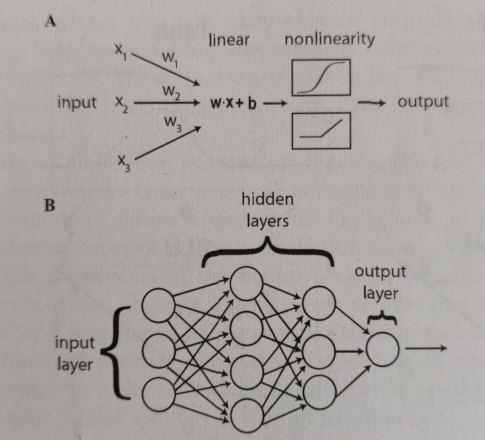
\includegraphics[width=0.7\linewidth]{gfx/Neuron}
	\caption{\itshape A) Neurons consist of a linear transformation that weights the importance of various inputs, followed by a non-linear activation function. B) Network architecture.}
	\label{fig:neuron}
\end{figure}




The linear transformation in almost all NNs takes the form of a dot product with a set of neuron-specific weights $\mw^{(i)} = (w^{(i)}_1,w^{(i)}_2,\dots,w^{(i)}_d)$ followed by re-centring with a neuron-specific bias $b^{(i)}$:
\be 
z^{(i)} = \mw^{(i)} \cdot \mx ü+ b^{(i)} = \textbf{x}^T \cdot \textbf{w}^{(i)},
\ee 
where $\textbf{x}=(1,\mx)$ and $\textbf{w}^{(i)} = (b^{(i)}, \mw^{(i)} )$.
\begin{mybox}{Choosing the right non-linearity}
 In terms of $z^{(i)}$ and the non-linear function $\sigma_i(z)$, we can write the full input-output function as 
\be 
\label{eq:dnnInputOutputfct}
a_i(\mx) = \sigma_i ( z^{(i)}).
\ee 
Historical choices of nonlinearities include step-functions (perceptrons), sigmoids (i.e. Fermi functions), and the hyperbolic tangent, cf. \ref{subsubsec:thresholdfct}. More recently, it has become more common to use rectified linear units (ReLUs), leaky rectified linear units (leaky ReLUs), and exponential linear units (ELUs). Different choice of non-linearities lead to different computational and training properties for neurons. The underlying reason for this is that we train neural nets using gd based methods, cf. \ref{sec:gd}, that require us to take derivatives of the neural input-output function with respect to the weights $\mw^{(i)}$ and the bias $b^{(i)}$.
\end{mybox}
Notice that the derivatives of the aforementioned non-linearities $\sigma(z)$ have very different properties. The derivative of the perceptron is zero everywhere except where the input is zero. This discontinuous behaviour makes it impossible to train perceptrons using gradient descent. For this reason, until recently the most popular choice of non-linearity was the $\tanh$ function or a sigmoid/Fermi function. However, this choice of non-linearity has a major drawback. When the input weights become large, as they often do in traingin, the activation functions saturates and the derivative of the output w.r.t. the weights tends to zero since $\partial \sigma /\partial z \rightarrow 0$ for $z\gg 1$. Such \emph{vanishing gradients} are a feature of any saturating function, making it harder to train deep networks. In contrast, for a non-saturating function such as ReLUs or ELUs, the gradients stay finite even for large inputs.

\subsubsection{Layering neurons to build deep networks: network architecture}
\label{subsubsec:dnnNetworkArchitecture}
The basic idea of all NNs is to layer neurons in a hierarchical fashion, the general structure of which is known as the \emph{network architecture}, compare \ref{fig:neuron}. In the simplest feed-forward networks, each neuron in the \emph{input layer} of the neurons takes the inputs $\textbf{x}$ and produces an output $a_i(\textbf{x})$ that depends on its current weights, see \ref{eq:dnnInputOutputfct}. The outputs of the input layer are then treated as the inputs to the next \emph{hidden layer}. This is usually repeated several times until one reaches the top or \emph{output layer}.
\begin{mybox}{Output layer and general architecture}
	The output layer is almost always a simple classifier of the form discussed before: a logistic regression \ref{sec:logisticRegression} or soft-max function \ref{subsec:logregSoftMax} in the case of categorical data (i.e. discrete labels) or a linear regression \ref{sec:linearRegression} layer in the case of continuous outputs. Thus, the whole neural network can be though of as a complicated nonlinear transformation of the inputs $\tx$ into an output $\hat{y}$ that depends on the weights and biases of all the neurons in the input, hidden, and output layers.
\end{mybox}
The use of hidden layers greatly expands the representation power (\emph{expressivity}) of a NN when compared with a simple soft-max or linear regression network, this is exemplified by the following theorem.
\begin{mybox}{Universal approximation theorem}
	A NN with a single hidden layer can approximate any continuous multi-input/multi-output function with arbitrary accuracy.
\end{mybox}
What does this mean and where does this come from ?\\
Note that by increasing the number of hidden neurons we can improve the approximation. Suppose we're given a function $f(x)$ which we'd like to compute to within some desired accuracy $ϵ>0$. The guarantee is that by using enough hidden neurons we can always find a neural network whose output $g(x)$ satisfies 
 \bse 
 \abs{g(x)-f(x)} < \epsilon,
 \ese 
  for all inputs $x$.
The approximation of the function works in the following way like a Riemann sum. Basically every pair of neurons in the hidden layer can be combined, via a combination of both weights, into a step function (or a sigmoid function which becomes a step function for large inputs). To be more precise, you can make every activation function into a step function by a clever combination of weights and bias if the activation function satisfies the following properties:\\
We do need to assume that $s(z)$ is well-defined as$z\rightarrow \infty$ and $z\rightarrow -\infty$. These two limits are the two values taken on by our step function. We also need to assume that these limits are different from one another. If they weren't, there'd be no step, simply a flat graph! But provided the activation function $s(z)$ satisfies these properties, neurons based on such an activation function are universal for computation (i.e. they are able to approximate any function).
\\
 Having $N$ pairs of hidden layer neuron pairs therefore gives you $N$ step function, which you can arrange beside each other, or overlapping. This is basically the approximation of the function. You Arrange step functions in such a way that they give you the function in a small section of the intervall. Therefore, basically neuron pairs in the hidden layer provide support functions as in analysis, which are step function approximating the true function for a small part of the interval. Therefore, by simply increasing the number of hidden layer neurons, you increase the number of step functions and decrease their width, resulting in a finer approximation of the function.\\
This makes use of the weighted combination $\sum_j w_j a_j$ output from the hidden neurons, however the function is given by the output layer, i.e. by the output $\sigma(\sum_j w_j a_j +b)$ where $b$ is the bias on the output neuron. How do you make the transition ?\\
The solution is to design a neural network whose hidden layer has a weighted output given by $\sigma^{-1}\circ f(x)$, such that the overall output will be a very good approximation of $\sigma\circ \sigma^{-1} \circ f(x) = f(x)$.
\\
If you have more inputs for one neuron, i.e. a many-input function $f(x_1,x_2,\dots)$, you get more weights, because every input $x_i$ has a weight $w_i$ associated with it which determines how much this input variable should contribute in this particular neuron, where every neuron also has one specific bias associated with it.\\
For two input variables:\\
 You can again create step function but this time in three dimensions (i.e. $x_1,x_2,g(x_1,x_2)$), which are called tower functions. These are constructed by introducing a second hidden layer. A pair of Neurons in the first hidden layer giving us a step-function in one direction can be combined with a pair of neurons giving us a step function in another direction (and so on) to create a tower function by a clever combination of heights of the two neuron pairs and bias of the neuron in the second hidden layer both of these pairs are connected to. Then, you can create any $3$ or $m$ dimensional function by stacking tower functions together. We can also make them as thin as we like, and whatever height we like. As a result, we can ensure that the weighted output from the second hidden layer approximates any desired function of two variables.
In particular, by making the weighted output from the second hidden layer a good approximation to $\sigma^{-1}\circ f$, we ensure the output from our network will be a good approximation to any desired function, $f$.\\
For $m$ input variables you need to have $m$ neuron pairs in the first hidden layer to feed into one respective neuron in the second hidden layer, where the former create all the step functions in the different dimensions by clever combination of parameters and the latter gives the output tower function in the given dimension.\\
For vector-valued functions, you simply compute the components of the vector separately via the above method and then put them into a vector.
\begin{mybox}{Conclusion}
We saw that we can approximate any function with just one hidden layer. Given this, you might wonder why we would ever be interested in deep networks, i.e., networks with many hidden layers. Can't we simply replace those networks with shallow, single hidden layer networks?\\
While in principle that's possible, there are good practical reasons to use deep networks. Deep networks have a hierarchical structure which makes them particularly well adapted to learn the hierarchies of knowledge that seem to be useful in solving real-world problems. Put more concretely, when attacking problems such as image recognition, it helps to use a system that understands not just individual pixels, but also increasingly more complex concepts: from edges to simple geometric shapes, all the way up through complex, multi-object scenes. Deep networks do a better job than shallow networks at learning such hierarchies of knowledge.
\end{mybox}
\subsubsection{Further on network architecture: How many layers is adequate for a problem ?}
\label{subsubsec:deepBestPracticeArchitecture}
Deep architectures are favourable for learning. Increasing the number of layers increases the number of parameters and hence the representational power of NNs. Indeed, recent numerical experiments suggest that as long as the number of parameters i larger than the number of data points, certain classes of NNs can fit arbitrarily labelled random noise samples. This suggests that large NNs of the kind used in practice can express highly complex function. Adding hidden layers is also though to allow neural nets to learn more complex features rom the data. Work on convolutional networks suggests that the first few layers of a neural network learn simple, ’low-level’ features thatare then combined into higher-level, more abstract features in the deeper layers.\\
\\
Choosing the exact network architecture for a NN remains an art that requires extensive numerical experimentation and intuition, and is often times problem-specific. Both the number of hidden layers and the number of neurons in each layer can affect the performance of a NN.
\begin{mybox}{Rule of thumb}
	A general rule of thumb that seems to be emerging is that the number of parameters in the NN should be large enough to prevent underfitting.
\end{mybox}
Empirically, the best architecture for a problem depends on the task, the amount and type of data that is available, and the computational resources at one's disposal. Certain architectures are easier to train, while others might be better at capturing complicated dependencies in the data and learning relevant input features. Finally, there architectures beyond simple deep, feed-forward NNs.
For example, modern NNs for image segmentation often incorporate ’skip connections’ that skip layers of NN. This allows information to directly propagate to a hidden or output layer, bypassing intermediate layers and often improving performance.

\subsubsection{Training deep networks}
\label{subsubsec:deepTraining}
\begin{mybox}{Training procedure}
	The training procedure is the same as we used for training simpler supervised learning algorithms such as logistic and linear regression, compare \ref{subsec:recipeML}:\\
	Construct a cost/loss function and then use gradient descent to minimize the cost function and find the optimal weights and biases. 
\end{mybox}
NNs differ from these simpler supervised procedures in that generally they contain multiple hidden layers that make taking the gradient computationally more difficult, this will be discussed in more detail via the \emph{backpropagation} algorithm for computing gradients in \ref{subsubsec:deepBackpropagation}.\\
\\
Like all supervised learning procedures, the first thing one must do to train a NN is to specify a loss function. Given a data point $(\tx_i,y_i)$, $\tx_i \in \mR^{d+1}$, the NN makes a prediction $\hat{y}_i(\tw)$, where $\tw$ are the parameters of the NN. Recall that in most cases, the top output layer of our NN is either a continuous predictor or a classifier that makes discrete (categorical) predictions. Depending on whether one wants to make continuous or categorical predictions, one must utilize a different kind of loss function.
\begin{enumerate} 
\item For continuous data, the loss functions that are commonly used to train NNs are identical to those used in linear regression:
\begin{enumerate}
	\item One is the mean squared error
	\be 
	\label{eq:deepCostSquaredError}
	E(\tw) = \frac{1}{n}\sum_{i=1}^n (y_i-\hat{y}_i(\tw) )^2, 
	\ee 
	where $n$ is the number of data points,
	\item and the mean-absolute error (i.e. $L_1$ norm) 
	\be 
	\label{eq:deepCostAbsoluteError} 
	E(\tw) = \frac{1}{n} \sum_i \abs{y_i - \hat{y}_i(\tw)}.
		\ee 
\end{enumerate}
The full cost function often includes terms that implement regularization (e.g. $L_1$ or $L_2$ regularizers).
\item For categorical data, the most commonly used loss function is the cross-entropy (\ref{eq:logregCrossEntropy} and \ref{eq:logregSoftMaxcostFct}), since the output layer is often taken to be a logistic classifier for binary data with two types of labels, or a soft-max classifier if there are more than two types of labels. As usual, these loss functions are often supplemented by aditional terms that implement regularization.
\end{enumerate}
Having defined an architecture and a cost function, we must now train the model. Similar to other supervised learning methods, we make use of gradient-descend based methods \ref{sec:gd} to optimize the cost function. Recall that the basic idea of GD is to update the parameters $\tw$ to move in the direction of the gradient of the cost function $\nabla_{\tw} E(\tw)$.\footnote{Most modern NN packages, such as Keras, allow te user to specify which of the optimizers discussed in \ref{sec:gd} they would like to use in order to train the NN. Depending on the architecture, data, and computation resources, different optimizers may work better on the problem, though vanilla SGD \ref{subsubsec:gdSGD} is a good first choice.}

\subsubsection{The Backpropagation algorithm}
\label{subsubsec:deepBackpropagation}








\chapter{Ideas for problems to work on}
\section{Physics problems}
\subsection{Cosmology}
\begin{enumerate}
	\item Maybe write a classification logistic regressor, or deep CNN to classify where dark matter halos have their boundary. It is very difficult to define a boundary of such a spread out object with confidence, maybe find criteria via classification ML technique ?
\end{enumerate}
\subsection{QFT}

\end{document}
% ********************************************************************
